% Copyright (c) Meta Platforms, Inc. and affiliates.

\documentclass{article}

\usepackage{neurips_2022}
% Copyright (c) Meta Platforms, Inc. and affiliates.

%%%%% NEW MATH DEFINITIONS %%%%%

\usepackage{amsmath,amsfonts,bm}

% Mark sections of captions for referring to divisions of figures
\newcommand{\figleft}{{\em (Left)}}
\newcommand{\figcenter}{{\em (Center)}}
\newcommand{\figright}{{\em (Right)}}
\newcommand{\figtop}{{\em (Top)}}
\newcommand{\figbottom}{{\em (Bottom)}}
\newcommand{\captiona}{{\em (a)}}
\newcommand{\captionb}{{\em (b)}}
\newcommand{\captionc}{{\em (c)}}
\newcommand{\captiond}{{\em (d)}}

% Highlight a newly defined term
\newcommand{\newterm}[1]{{\bf #1}}


% Figure reference, lower-case.
\def\figref#1{figure~\ref{#1}}
% Figure reference, capital. For start of sentence
\def\Figref#1{Figure~\ref{#1}}
\def\twofigref#1#2{figures \ref{#1} and \ref{#2}}
\def\quadfigref#1#2#3#4{figures \ref{#1}, \ref{#2}, \ref{#3} and \ref{#4}}
% Section reference, lower-case.
\def\secref#1{section~\ref{#1}}
% Section reference, capital.
\def\Secref#1{Section~\ref{#1}}
% Reference to two sections.
\def\twosecrefs#1#2{sections \ref{#1} and \ref{#2}}
% Reference to three sections.
\def\secrefs#1#2#3{sections \ref{#1}, \ref{#2} and \ref{#3}}
% Reference to an equation, lower-case.
\def\eqref#1{equation~\ref{#1}}
% Reference to an equation, upper case
\def\Eqref#1{Equation~\ref{#1}}
% A raw reference to an equation---avoid using if possible
\def\plaineqref#1{\ref{#1}}
% Reference to a chapter, lower-case.
\def\chapref#1{chapter~\ref{#1}}
% Reference to an equation, upper case.
\def\Chapref#1{Chapter~\ref{#1}}
% Reference to a range of chapters
\def\rangechapref#1#2{chapters\ref{#1}--\ref{#2}}
% Reference to an algorithm, lower-case.
\def\algref#1{algorithm~\ref{#1}}
% Reference to an algorithm, upper case.
\def\Algref#1{Algorithm~\ref{#1}}
\def\twoalgref#1#2{algorithms \ref{#1} and \ref{#2}}
\def\Twoalgref#1#2{Algorithms \ref{#1} and \ref{#2}}
% Reference to a part, lower case
\def\partref#1{part~\ref{#1}}
% Reference to a part, upper case
\def\Partref#1{Part~\ref{#1}}
\def\twopartref#1#2{parts \ref{#1} and \ref{#2}}

\def\ceil#1{\lceil #1 \rceil}
\def\floor#1{\lfloor #1 \rfloor}
\def\1{\bm{1}}
\newcommand{\train}{\mathcal{D}}
\newcommand{\valid}{\mathcal{D_{\mathrm{valid}}}}
\newcommand{\test}{\mathcal{D_{\mathrm{test}}}}

\def\eps{{\epsilon}}


% Random variables
\def\reta{{\textnormal{$\eta$}}}
\def\ra{{\textnormal{a}}}
\def\rb{{\textnormal{b}}}
\def\rc{{\textnormal{c}}}
\def\rd{{\textnormal{d}}}
\def\re{{\textnormal{e}}}
\def\rf{{\textnormal{f}}}
\def\rg{{\textnormal{g}}}
\def\rh{{\textnormal{h}}}
\def\ri{{\textnormal{i}}}
\def\rj{{\textnormal{j}}}
\def\rk{{\textnormal{k}}}
\def\rl{{\textnormal{l}}}
% rm is already a command, just don't name any random variables m
\def\rn{{\textnormal{n}}}
\def\ro{{\textnormal{o}}}
\def\rp{{\textnormal{p}}}
\def\rq{{\textnormal{q}}}
\def\rr{{\textnormal{r}}}
\def\rs{{\textnormal{s}}}
\def\rt{{\textnormal{t}}}
\def\ru{{\textnormal{u}}}
\def\rv{{\textnormal{v}}}
\def\rw{{\textnormal{w}}}
\def\rx{{\textnormal{x}}}
\def\ry{{\textnormal{y}}}
\def\rz{{\textnormal{z}}}

% Random vectors
\def\rvepsilon{{\mathbf{\epsilon}}}
\def\rvtheta{{\mathbf{\theta}}}
\def\rva{{\mathbf{a}}}
\def\rvb{{\mathbf{b}}}
\def\rvc{{\mathbf{c}}}
\def\rvd{{\mathbf{d}}}
\def\rve{{\mathbf{e}}}
\def\rvf{{\mathbf{f}}}
\def\rvg{{\mathbf{g}}}
\def\rvh{{\mathbf{h}}}
\def\rvu{{\mathbf{i}}}
\def\rvj{{\mathbf{j}}}
\def\rvk{{\mathbf{k}}}
\def\rvl{{\mathbf{l}}}
\def\rvm{{\mathbf{m}}}
\def\rvn{{\mathbf{n}}}
\def\rvo{{\mathbf{o}}}
\def\rvp{{\mathbf{p}}}
\def\rvq{{\mathbf{q}}}
\def\rvr{{\mathbf{r}}}
\def\rvs{{\mathbf{s}}}
\def\rvt{{\mathbf{t}}}
\def\rvu{{\mathbf{u}}}
\def\rvv{{\mathbf{v}}}
\def\rvw{{\mathbf{w}}}
\def\rvx{{\mathbf{x}}}
\def\rvy{{\mathbf{y}}}
\def\rvz{{\mathbf{z}}}

% Elements of random vectors
\def\erva{{\textnormal{a}}}
\def\ervb{{\textnormal{b}}}
\def\ervc{{\textnormal{c}}}
\def\ervd{{\textnormal{d}}}
\def\erve{{\textnormal{e}}}
\def\ervf{{\textnormal{f}}}
\def\ervg{{\textnormal{g}}}
\def\ervh{{\textnormal{h}}}
\def\ervi{{\textnormal{i}}}
\def\ervj{{\textnormal{j}}}
\def\ervk{{\textnormal{k}}}
\def\ervl{{\textnormal{l}}}
\def\ervm{{\textnormal{m}}}
\def\ervn{{\textnormal{n}}}
\def\ervo{{\textnormal{o}}}
\def\ervp{{\textnormal{p}}}
\def\ervq{{\textnormal{q}}}
\def\ervr{{\textnormal{r}}}
\def\ervs{{\textnormal{s}}}
\def\ervt{{\textnormal{t}}}
\def\ervu{{\textnormal{u}}}
\def\ervv{{\textnormal{v}}}
\def\ervw{{\textnormal{w}}}
\def\ervx{{\textnormal{x}}}
\def\ervy{{\textnormal{y}}}
\def\ervz{{\textnormal{z}}}

% Random matrices
\def\rmA{{\mathbf{A}}}
\def\rmB{{\mathbf{B}}}
\def\rmC{{\mathbf{C}}}
\def\rmD{{\mathbf{D}}}
\def\rmE{{\mathbf{E}}}
\def\rmF{{\mathbf{F}}}
\def\rmG{{\mathbf{G}}}
\def\rmH{{\mathbf{H}}}
\def\rmI{{\mathbf{I}}}
\def\rmJ{{\mathbf{J}}}
\def\rmK{{\mathbf{K}}}
\def\rmL{{\mathbf{L}}}
\def\rmM{{\mathbf{M}}}
\def\rmN{{\mathbf{N}}}
\def\rmO{{\mathbf{O}}}
\def\rmP{{\mathbf{P}}}
\def\rmQ{{\mathbf{Q}}}
\def\rmR{{\mathbf{R}}}
\def\rmS{{\mathbf{S}}}
\def\rmT{{\mathbf{T}}}
\def\rmU{{\mathbf{U}}}
\def\rmV{{\mathbf{V}}}
\def\rmW{{\mathbf{W}}}
\def\rmX{{\mathbf{X}}}
\def\rmY{{\mathbf{Y}}}
\def\rmZ{{\mathbf{Z}}}

% Elements of random matrices
\def\ermA{{\textnormal{A}}}
\def\ermB{{\textnormal{B}}}
\def\ermC{{\textnormal{C}}}
\def\ermD{{\textnormal{D}}}
\def\ermE{{\textnormal{E}}}
\def\ermF{{\textnormal{F}}}
\def\ermG{{\textnormal{G}}}
\def\ermH{{\textnormal{H}}}
\def\ermI{{\textnormal{I}}}
\def\ermJ{{\textnormal{J}}}
\def\ermK{{\textnormal{K}}}
\def\ermL{{\textnormal{L}}}
\def\ermM{{\textnormal{M}}}
\def\ermN{{\textnormal{N}}}
\def\ermO{{\textnormal{O}}}
\def\ermP{{\textnormal{P}}}
\def\ermQ{{\textnormal{Q}}}
\def\ermR{{\textnormal{R}}}
\def\ermS{{\textnormal{S}}}
\def\ermT{{\textnormal{T}}}
\def\ermU{{\textnormal{U}}}
\def\ermV{{\textnormal{V}}}
\def\ermW{{\textnormal{W}}}
\def\ermX{{\textnormal{X}}}
\def\ermY{{\textnormal{Y}}}
\def\ermZ{{\textnormal{Z}}}

% Vectors
\def\vzero{{\bm{0}}}
\def\vone{{\bm{1}}}
\def\vmu{{\bm{\mu}}}
\def\vtheta{{\bm{\theta}}}
\def\va{{\bm{a}}}
\def\vb{{\bm{b}}}
\def\vc{{\bm{c}}}
\def\vd{{\bm{d}}}
\def\ve{{\bm{e}}}
\def\vf{{\bm{f}}}
\def\vg{{\bm{g}}}
\def\vh{{\bm{h}}}
\def\vi{{\bm{i}}}
\def\vj{{\bm{j}}}
\def\vk{{\bm{k}}}
\def\vl{{\bm{l}}}
\def\vm{{\bm{m}}}
\def\vn{{\bm{n}}}
\def\vo{{\bm{o}}}
\def\vp{{\bm{p}}}
\def\vq{{\bm{q}}}
\def\vr{{\bm{r}}}
\def\vs{{\bm{s}}}
\def\vt{{\bm{t}}}
\def\vu{{\bm{u}}}
\def\vv{{\bm{v}}}
\def\vw{{\bm{w}}}
\def\vx{{\bm{x}}}
\def\vy{{\bm{y}}}
\def\vz{{\bm{z}}}

% Elements of vectors
\def\evalpha{{\alpha}}
\def\evbeta{{\beta}}
\def\evepsilon{{\epsilon}}
\def\evlambda{{\lambda}}
\def\evomega{{\omega}}
\def\evmu{{\mu}}
\def\evpsi{{\psi}}
\def\evsigma{{\sigma}}
\def\evtheta{{\theta}}
\def\eva{{a}}
\def\evb{{b}}
\def\evc{{c}}
\def\evd{{d}}
\def\eve{{e}}
\def\evf{{f}}
\def\evg{{g}}
\def\evh{{h}}
\def\evi{{i}}
\def\evj{{j}}
\def\evk{{k}}
\def\evl{{l}}
\def\evm{{m}}
\def\evn{{n}}
\def\evo{{o}}
\def\evp{{p}}
\def\evq{{q}}
\def\evr{{r}}
\def\evs{{s}}
\def\evt{{t}}
\def\evu{{u}}
\def\evv{{v}}
\def\evw{{w}}
\def\evx{{x}}
\def\evy{{y}}
\def\evz{{z}}

% Matrix
\def\mA{{\bm{A}}}
\def\mB{{\bm{B}}}
\def\mC{{\bm{C}}}
\def\mD{{\bm{D}}}
\def\mE{{\bm{E}}}
\def\mF{{\bm{F}}}
\def\mG{{\bm{G}}}
\def\mH{{\bm{H}}}
\def\mI{{\bm{I}}}
\def\mJ{{\bm{J}}}
\def\mK{{\bm{K}}}
\def\mL{{\bm{L}}}
\def\mM{{\bm{M}}}
\def\mN{{\bm{N}}}
\def\mO{{\bm{O}}}
\def\mP{{\bm{P}}}
\def\mQ{{\bm{Q}}}
\def\mR{{\bm{R}}}
\def\mS{{\bm{S}}}
\def\mT{{\bm{T}}}
\def\mU{{\bm{U}}}
\def\mV{{\bm{V}}}
\def\mW{{\bm{W}}}
\def\mX{{\bm{X}}}
\def\mY{{\bm{Y}}}
\def\mZ{{\bm{Z}}}
\def\mBeta{{\bm{\beta}}}
\def\mPhi{{\bm{\Phi}}}
\def\mLambda{{\bm{\Lambda}}}
\def\mSigma{{\bm{\Sigma}}}

% Tensor
\DeclareMathAlphabet{\mathsfit}{\encodingdefault}{\sfdefault}{m}{sl}
\SetMathAlphabet{\mathsfit}{bold}{\encodingdefault}{\sfdefault}{bx}{n}
\newcommand{\tens}[1]{\bm{\mathsfit{#1}}}
\def\tA{{\tens{A}}}
\def\tB{{\tens{B}}}
\def\tC{{\tens{C}}}
\def\tD{{\tens{D}}}
\def\tE{{\tens{E}}}
\def\tF{{\tens{F}}}
\def\tG{{\tens{G}}}
\def\tH{{\tens{H}}}
\def\tI{{\tens{I}}}
\def\tJ{{\tens{J}}}
\def\tK{{\tens{K}}}
\def\tL{{\tens{L}}}
\def\tM{{\tens{M}}}
\def\tN{{\tens{N}}}
\def\tO{{\tens{O}}}
\def\tP{{\tens{P}}}
\def\tQ{{\tens{Q}}}
\def\tR{{\tens{R}}}
\def\tS{{\tens{S}}}
\def\tT{{\tens{T}}}
\def\tU{{\tens{U}}}
\def\tV{{\tens{V}}}
\def\tW{{\tens{W}}}
\def\tX{{\tens{X}}}
\def\tY{{\tens{Y}}}
\def\tZ{{\tens{Z}}}


% Graph
\def\gA{{\mathcal{A}}}
\def\gB{{\mathcal{B}}}
\def\gC{{\mathcal{C}}}
\def\gD{{\mathcal{D}}}
\def\gE{{\mathcal{E}}}
\def\gF{{\mathcal{F}}}
\def\gG{{\mathcal{G}}}
\def\gH{{\mathcal{H}}}
\def\gI{{\mathcal{I}}}
\def\gJ{{\mathcal{J}}}
\def\gK{{\mathcal{K}}}
\def\gL{{\mathcal{L}}}
\def\gM{{\mathcal{M}}}
\def\gN{{\mathcal{N}}}
\def\gO{{\mathcal{O}}}
\def\gP{{\mathcal{P}}}
\def\gQ{{\mathcal{Q}}}
\def\gR{{\mathcal{R}}}
\def\gS{{\mathcal{S}}}
\def\gT{{\mathcal{T}}}
\def\gU{{\mathcal{U}}}
\def\gV{{\mathcal{V}}}
\def\gW{{\mathcal{W}}}
\def\gX{{\mathcal{X}}}
\def\gY{{\mathcal{Y}}}
\def\gZ{{\mathcal{Z}}}

% Sets
\def\sA{{\mathbb{A}}}
\def\sB{{\mathbb{B}}}
\def\sC{{\mathbb{C}}}
\def\sD{{\mathbb{D}}}
% Don't use a set called E, because this would be the same as our symbol
% for expectation.
\def\sF{{\mathbb{F}}}
\def\sG{{\mathbb{G}}}
\def\sH{{\mathbb{H}}}
\def\sI{{\mathbb{I}}}
\def\sJ{{\mathbb{J}}}
\def\sK{{\mathbb{K}}}
\def\sL{{\mathbb{L}}}
\def\sM{{\mathbb{M}}}
\def\sN{{\mathbb{N}}}
\def\sO{{\mathbb{O}}}
\def\sP{{\mathbb{P}}}
\def\sQ{{\mathbb{Q}}}
\def\sR{{\mathbb{R}}}
\def\sS{{\mathbb{S}}}
\def\sT{{\mathbb{T}}}
\def\sU{{\mathbb{U}}}
\def\sV{{\mathbb{V}}}
\def\sW{{\mathbb{W}}}
\def\sX{{\mathbb{X}}}
\def\sY{{\mathbb{Y}}}
\def\sZ{{\mathbb{Z}}}

% Entries of a matrix
\def\emLambda{{\Lambda}}
\def\emA{{A}}
\def\emB{{B}}
\def\emC{{C}}
\def\emD{{D}}
\def\emE{{E}}
\def\emF{{F}}
\def\emG{{G}}
\def\emH{{H}}
\def\emI{{I}}
\def\emJ{{J}}
\def\emK{{K}}
\def\emL{{L}}
\def\emM{{M}}
\def\emN{{N}}
\def\emO{{O}}
\def\emP{{P}}
\def\emQ{{Q}}
\def\emR{{R}}
\def\emS{{S}}
\def\emT{{T}}
\def\emU{{U}}
\def\emV{{V}}
\def\emW{{W}}
\def\emX{{X}}
\def\emY{{Y}}
\def\emZ{{Z}}
\def\emSigma{{\Sigma}}

% entries of a tensor
% Same font as tensor, without \bm wrapper
\newcommand{\etens}[1]{\mathsfit{#1}}
\def\etLambda{{\etens{\Lambda}}}
\def\etA{{\etens{A}}}
\def\etB{{\etens{B}}}
\def\etC{{\etens{C}}}
\def\etD{{\etens{D}}}
\def\etE{{\etens{E}}}
\def\etF{{\etens{F}}}
\def\etG{{\etens{G}}}
\def\etH{{\etens{H}}}
\def\etI{{\etens{I}}}
\def\etJ{{\etens{J}}}
\def\etK{{\etens{K}}}
\def\etL{{\etens{L}}}
\def\etM{{\etens{M}}}
\def\etN{{\etens{N}}}
\def\etO{{\etens{O}}}
\def\etP{{\etens{P}}}
\def\etQ{{\etens{Q}}}
\def\etR{{\etens{R}}}
\def\etS{{\etens{S}}}
\def\etT{{\etens{T}}}
\def\etU{{\etens{U}}}
\def\etV{{\etens{V}}}
\def\etW{{\etens{W}}}
\def\etX{{\etens{X}}}
\def\etY{{\etens{Y}}}
\def\etZ{{\etens{Z}}}

% The true underlying data generating distribution
\newcommand{\pdata}{p_{\rm{data}}}
% The empirical distribution defined by the training set
\newcommand{\ptrain}{\hat{p}_{\rm{data}}}
\newcommand{\Ptrain}{\hat{P}_{\rm{data}}}
% The model distribution
\newcommand{\pmodel}{p_{\rm{model}}}
\newcommand{\Pmodel}{P_{\rm{model}}}
\newcommand{\ptildemodel}{\tilde{p}_{\rm{model}}}
% Stochastic autoencoder distributions
\newcommand{\pencode}{p_{\rm{encoder}}}
\newcommand{\pdecode}{p_{\rm{decoder}}}
\newcommand{\precons}{p_{\rm{reconstruct}}}
\newcommand{\sam}[1]{{\color{blue}{\bf[Sam:} #1{\bf]}}}

\newcommand{\laplace}{\mathrm{Laplace}} % Laplace distribution

\newcommand{\E}{\mathop{\mathbb{E}}}
\newcommand{\Ls}{\mathcal{L}}
\newcommand{\R}{\mathbb{R}}
\newcommand{\emp}{\tilde{p}}
\newcommand{\lr}{\alpha}
\newcommand{\reg}{\lambda}
\newcommand{\rect}{\mathrm{rectifier}}
\newcommand{\softmax}{\mathrm{softmax}}
\newcommand{\sigmoid}{\sigma}
\newcommand{\softplus}{\zeta}
\newcommand{\KL}{D_{\mathrm{KL}}}
\newcommand{\Var}{\mathrm{Var}}
\newcommand{\standarderror}{\mathrm{SE}}
\newcommand{\Cov}{\mathrm{Cov}}
% Wolfram Mathworld says $L^2$ is for function spaces and $\ell^2$ is for vectors
% But then they seem to use $L^2$ for vectors throughout the site, and so does
% wikipedia.
\newcommand{\normlzero}{L^0}
\newcommand{\normlone}{L^1}
\newcommand{\normltwo}{L^2}
\newcommand{\normlp}{L^p}
\newcommand{\normmax}{L^\infty}

\newcommand{\parents}{Pa} % See usage in notation.tex. Chosen to match Daphne's book.

\DeclareMathOperator*{\argmax}{arg\,max}
\DeclareMathOperator*{\argmin}{arg\,min}
\DeclareMathOperator*{\subjectto}{subject\;to}
\DeclareMathOperator*{\where}{where}
\DeclareMathOperator*{\proj}{proj}

\DeclareMathOperator{\sign}{sign}
\DeclareMathOperator{\Tr}{Tr}
\let\ab\allowbreak


\usepackage[utf8]{inputenc}
\usepackage[T1]{fontenc}
\usepackage{textcomp}
\usepackage{float}
\usepackage[normalem]{ulem}

\usepackage{graphicx}
\usepackage{booktabs}
\usepackage{diagbox}
\usepackage{wrapfig}
\usepackage{numprint}

\usepackage{listings}
\lstset{
  language=bash,frame=single, numbers=left,numbersep=5pt,
  numberstyle=\tiny\color{black!80},
  basicstyle=\footnotesize\ttfamily,
  commentstyle=\itshape\color{blue!50},
  backgroundcolor=\color{gray!10!white},
  breaklines=true
}

\usepackage[table,svgnames]{xcolor}
\definecolor{linkcolor}{RGB}{74, 102, 146}
\newcommand{\cellhi}{\cellcolor{RoyalBlue!15}}
\usepackage[colorlinks=true,allcolors=linkcolor,pageanchor=true,plainpages=false,pdfpagelabels,bookmarks,bookmarksnumbered]{hyperref}
\usepackage{transparent}

\usepackage{graphicx}
\usepackage{hyperref}
\usepackage{url}

\usepackage[edges]{forest}

\usepackage{algpseudocode}
\algnewcommand{\LeftCommentX}[1]{\Statex \(\triangleright\) #1}
\algnewcommand{\LeftComment}[1]{\State \(\triangleright\) #1}

\usepackage{tikz}
\usetikzlibrary{arrows,backgrounds,bayesnet,calc,matrix}

\newcommand{\cblock}[3]{
  \hspace{-1.5mm}
  \begin{tikzpicture}[node/.style={square, minimum size=10mm, thick, line width=0pt}]
    \node[fill={rgb,255:red,#1;green,#2;blue,#3}] () [] {};
  \end{tikzpicture}%
}

\newcommand{\circlegend}[2]{
  \hspace{-1.5mm}
  \begin{tikzpicture}[node/.style={square, minimum size=10mm, thick, line width=0pt}]
    \node[circle,fill={#1},draw=black,thick] (block) [] {};
    \node[right=0mm of block,yshift=-.3mm] {#2};
  \end{tikzpicture}%
}

\usepackage{algorithm, algpseudocode}

\usepackage[nameinlink]{cleveref}
\Crefname{equation}{Eq.}{Eqs.}
\Crefname{section}{Sect.}{Sects.}
\Crefname{appendix}{App.}{Apps.}
\Crefname{definition}{Def.}{Defs.}
\Crefname{proposition}{Prop.}{Props.}

\usepackage{xspace}
\newcommand{\eg}{e.g.\xspace}
\newcommand{\ie}{i.e.\xspace}

\usepackage{mathtools}
\newcommand{\defeq}{\vcentcolon=}

\usepackage{xspace}
\definecolor{bdacolor}{RGB}{168, 141, 201}
\newcommand{\bda}[1]{\textcolor{bdacolor}{[bda: #1]}}
\newcommand{\giulia}[1]{\textcolor{purple}{Giulia: #1}}
\newcommand{\ievgen}[1]{\textcolor{blue}{[Ievgen: #1]}}

\usepackage{todonotes}
\newcommand{\todon}[1]{\todo[color=red!40,inline,size=\small]{TODO: #1}}
\newcommand{\todoc}{\todo[color=red!40,inline,size=\small]{TODO: Complete}}
\newcommand{\todorw}{\todo[color=red!40,inline,size=\small]{TODO: Re-write}}
\newcommand{\todoi}[1]{{\color{red} [TODO] #1}\xspace}

\usepackage[misc]{ifsym} % \Letter
\usepackage[symbol]{footmisc}
\renewcommand{\thefootnote}{\fnsymbol{footnote}}

\begin{document}

\title{Meta Optimal Transport}
\author{Brandon Amos$^{1\;\textrm{\normalfont\Letter}}$\qquad \stepcounter{footnote}Samuel Cohen$^{12}$\thanks{Contributed while at UCL and visiting Meta AI.}\qquad Giulia Luise$^2$\qquad Ievgen Redko$^{34}$ \\
  $^1$Meta AI\quad $^2$University College London\quad $^3$University Jean Monnet\quad $^4$Aalto University \\
  $^\textrm{\Letter}$\hspace{0.5mm}Correspondence to: \texttt{bda@meta.com}}
\maketitle

\begin{abstract}
  We study the use of amortized optimization to predict optimal transport (OT) maps
  from the input measures, which we call \emph{Meta OT}.
  This helps repeatedly solve similar OT problems between different
  measures by leveraging the knowledge and information present
  from past problems to rapidly predict and solve new problems.
  Otherwise, standard methods ignore the knowledge of the
  past solutions and suboptimally re-solve each problem from scratch.
  Meta OT models surpass the standard
  convergence rates of log-Sinkhorn solvers in the discrete setting
  and convex potentials in the continuous setting.
  We improve the computational time of standard OT solvers
  by multiple orders of magnitude in discrete and continuous
  transport settings between images, spherical data, and color palettes.
  Our source code is available at \url{http://github.com/facebookresearch/meta-ot}.
\end{abstract}

\section{Introduction}
Optimal transportation \citep{villani2009optimal,ambrosio2003lecture,santambrogio2015optimal,peyre2019computational,merigot2021optimal} is thriving in domains including
economics \citep{galichon2016optimal},
reinforcement learning \citep{dadashi2020primal,fickinger2021cross},
style transfer \citep{kolkin2019style},
generative modeling \citep{arjovsky2017wasserstein,seguy2017large,huang2020convex,rout2021generative},
geometry \citep{solomon2015convolutional,cohen2021riemannian},
domain adaptation \citep{courty2017joint,redko2019optimal},
signal processing \citep{kolouri2017optimal},
fairness \citep{jiang2020wasserstein}, and cell reprogramming \citep{SCHIEBINGER2019928}.
A core component in these settings is to couple two
measures $(\alpha,\beta)$ supported on domains $(\gX, \gY)$
by solving a transport optimization problem such as the
\emph{primal Kantorovich problem}, which is defined by:
\begin{equation}
  \pi^\star(\alpha, \beta, c)\in \argmin_{\pi\in\gU(\alpha, \beta)}
    \int_{\gX\times \gY} c(x,y){\rm d}\pi(x,y),
  \label{eq:kantorovich-primal}
\end{equation}
where the \emph{optimal coupling} $\pi^\star$
is a joint distribution over the  product space,
$\gU(\alpha, \beta)$ is the set of admissible couplings
between $\alpha$ and $\beta$, and
$c: \gX\times\gY \rightarrow \R$ is the \emph{ground cost}, that represents a notion of distance between elements in $\mathcal{X}$ and elements in $\mathcal{Y}$.

\textbf{Challenges.}
Unfortunately, solving \cref{eq:kantorovich-primal} \emph{once} is
computationally expensive between general measures  and
computationally cheaper alternatives are an active research topic:
\emph{Entropic optimal transport} \citep{cuturi2013sinkhorn}
smooths the transport problem with an entropy penalty, and
\emph{sliced distances}
\citep{kolouri2016sliced,kolouri2018sliced,kolouri2019generalized,deshpande2019max}
solve OT between 1-dimensional projections of the measures,
where \cref{eq:kantorovich-primal} can be solved easily.

Furthermore, when an optimal transport method is deployed
in practice, \cref{eq:kantorovich-primal} is not just solved a
single time, but is \emph{repeatedly} solved for new
scenarios between different input measures $(\alpha, \beta)$.
For example, the measures could be representations of images
we care about optimally transporting between and in deployment
we would receive a stream of new images to couple.
Standard optimal transport solvers deployed in this
setting would re-solve the optimization problems from
scratch, but this ignores the shared structure and
information present between different coupling problems.
We note this is \emph{not} the out-of-sample setting
of \citet{seguy2017large,perrot2016mapping} that
seeks to couple measures and then extrapolate the map to
larger measures containing the original measures.

\textbf{Overview and outline.}
We study the use of amortized optimization and machine learning
methods to rapidly solve multiple optimal transport problems
and predict the solution from the input measures $(\alpha, \beta)$.
This setting involves learning a \emph{meta} model
to predict the solution to the optimal transport problem,
which we will refer to as \emph{Meta Optimal Transport}.
We learn Meta OT models to predict the solutions to optimal
transport problems and significantly improve the computational
time and number of iterations needed to solve
\cref{eq:kantorovich-primal} between
discrete (\cref{sec:meta-ot:discrete}) and
continuous (\cref{sec:meta-ot:icnn}) measures. The paper is organized
as follows: \cref{sec:preliminaries_andback} recalls the main
concepts needed for the rest of the paper, in particular the
formulations of the entropy regularized and unregularized optimal
transport problems and the basic notions of amortized optimization;
\cref{sec:meta} presents the Meta OT models and algorithms; and
\cref{sec:experiments} empirically demonstrates the
effectiveness of Meta OT.

\section{Preliminaries and background}\label{sec:preliminaries_andback}
\subsection{Dual optimal transport solvers}
We review foundations of optimal transportation, following
the notation of \citet{peyre2019computational} in most places.
The discrete setting often favors the entropic
regularized version since it can be computed efficiently
and in a parallelized way using the Sinkhorn algorithm.
On the other hand, the continuous setting is often solved from
samples using convex potentials.
While the primal Kantorovich formulation in \cref{eq:kantorovich-primal}
provides an intuitive problem description, optimal transport problems
are rarely solved directly in this form due to the high-dimensionality
of the couplings $\pi$ and the difficulty of satisfying the
coupling constraints $\gU(\alpha, \beta)$.
Instead, most computational OT solvers use the \emph{dual} of \cref{eq:kantorovich-primal},
which we build our
Meta OT solvers on top of in discrete and continuous settings.
\looseness=-1

\subsubsection{Entropic OT between discrete measures with the Sinkhorn algorithm}
\label{sec:prelim:discrete}

\begin{wrapfigure}{R}{0.5\textwidth}
  \vspace{-11mm}
  \begin{minipage}{0.5\textwidth}
    \begin{algorithm}[H]
      \caption{\footnotesize Sinkhorn($\alpha, \beta, c, \epsilon, f_0=0$)}
      \begin{algorithmic}
        \footnotesize
        \For {iteration $i$ = 1 to $N$}
        \State $g_{i} \leftarrow \epsilon \log b - \epsilon\log\left(
          K^\top \exp\{f_{i-1}/\epsilon\}\right)$
        \State $f_{i} \leftarrow \epsilon \log a - \epsilon\log\left(
          K \exp\{g_i/\epsilon\}\right)$
        \EndFor
        \State Compute $P_N$ from $f_N,g_N$ using \cref{eq:entropic-duals-to-primal}
        \State\Return $P_N\approx P^\star$
      \end{algorithmic}
      \label{alg:sinkhorn}
    \end{algorithm}
  \end{minipage}
  \vspace{-6mm}
\end{wrapfigure}
Let $\alpha\defeq\sum_{i=1}^m a_i\delta_{x_i}$ and
$\beta\defeq\sum_{i=1}^n b_i\delta_{y_i}$
be
\emph{discrete} measures,
where $\delta_z$ is a Dirac at point $z$
and $a\in\Delta_{m-1}$ and $b\in\Delta_{n-1}$ are
in the \emph{probability simplex} defined by
\begin{equation}
  \label{eq:simplex}
  \Delta_{k-1}\defeq\{x\in \R^k : x\geq 0\; {\rm and}\; \sum_i x_i=1\}.
  \footnotesize
\end{equation}

\textbf{Discrete OT.}
In the discrete setting,
\cref{eq:kantorovich-primal} simplifies to the \emph{linear program}
\begin{equation}
  P^\star(\alpha,\beta,c)\in \argmin_{P\in U(a,b)} \langle C, P \rangle \qquad
  U(a, b)\defeq \{P\in\R_+^{n\times m} : P 1_m = a,\quad P^\top 1_n = b\}
  \label{eq:discrete-primal}
\end{equation}
where $P$ is a \emph{coupling matrix},
$P^\star(\alpha, \beta)$ is the \emph{optimal} coupling,
and the \emph{cost} can be discretized as a matrix $C\in\R^{m\times n}$ with entries
$C_{i,j}\defeq c(x_i, y_j)$, and
$\langle C, P\rangle \defeq \sum_{i,j}C_{i,j}P_{i,j}$,

\textbf{Entropic OT.}
The linear program above can be regularized adding the entropy
of the coupling to smooth the objective as in
\citet{cominetti1994asymptotic,cuturi2013sinkhorn},
resulting in:
\begin{equation}
  P^\star(\alpha,\beta,c,\epsilon)\in \argmin_{P\in U(a,b)} \langle C, P \rangle - \epsilon H(P)
  \label{eq:entropic-primal}
\end{equation}
where $H(P)\defeq -\sum_{i,j} P_{i,j}(\log(P_{i,j})-1)$
is the discrete entropy of a coupling matrix $P$.

\textbf{Entropic OT dual.}
As presented in \citet[Prop.~4.4]{peyre2019computational},
the dual of \cref{eq:entropic-primal} is
\begin{equation}
  f^\star,g^\star\in\argmax_{f\in\R^n,g\in\R^m} \langle f, a\rangle + \langle g, b \rangle
    - \epsilon\left\langle \exp\{f/\epsilon\}, K\exp\{g/\epsilon\}\right\rangle,
  \quad
  K_{i,j}\defeq \exp\{-C_{i,j}/\epsilon\},
  \label{eq:entropic-dual}
\end{equation}
where $K\in\R^{m\times n}$ is the \emph{Gibbs kernel}
and the \emph{dual variables} or \emph{potentials}
$f\in\R^n$ and $g\in\R^m$ are associated, respectively, with the
marginal constraints $P1_m=a$ and $P^\top 1_n=b$.
The optimal duals depend on the problem,
\eg $f^\star(\alpha, \beta, c, \epsilon)$, but we
omit this dependence for notational simplicity.

\textbf{Recovering the primal solution from the duals.}
Given optimal duals $f^\star$, $g^\star$ that solve
\cref{eq:entropic-dual} the optimal coupling
$P^\star$ to the primal problem in \cref{eq:entropic-primal}
can be obtained by
\begin{equation}
  P_{i,j}^\star(\alpha, \beta, c, \epsilon)\defeq \exp\{f_i^\star/\epsilon\}K_{i,j}\exp\{g_j^\star/\epsilon\}
  \qquad
  (K\ {\rm is\ defined\ in\ \cref{eq:entropic-dual}})
  \label{eq:entropic-duals-to-primal}
\end{equation}

\textbf{The Sinkhorn algorithm}.
\Cref{alg:sinkhorn} summarizes the log-space version,
which takes closed-form block coordinate ascent updates
on \cref{eq:entropic-dual}
obtained from the first-order optimality conditions
\citep[Remark~4.21]{peyre2019computational}.
We will use it to fine-tune predictions made
by our Meta OT models.

\textbf{Computing the error.}
Standard implementations of the Sinkhorn algorithm,
such as \citet{flamary2021pot,cuturi2022optimal},
measure the error of a candidate dual solution $(f,g)$ by
computing the deviation from the marginal constraints,
which we will also use in comparing our solution quality:
\begin{equation}
  {\rm err}(f,g; \alpha, \beta, c)\defeq\|P1_m-a\|_1 + \|P^\top1_n-b\|_1
  \qquad
  {\rm (compute}\ P\ {\rm from\ \cref{eq:entropic-duals-to-primal})}
  \label{eq:sinkhorn-err}
\end{equation}

\textbf{Mapping between the duals.}
The first-order optimality conditions of \cref{eq:entropic-dual}
also provide an equivalence between the optimal dual potentials
that we will make use of:
\begin{equation}
  g(f; b, c) \defeq \epsilon \log b - \epsilon\log\left(
    K^\top \exp\{f/\epsilon\}\right).
  \label{eq:f-to-g}
\end{equation}


\subsubsection{Wasserstein-2 OT between continuous (Euclidean) measures with dual potentials}
\label{sec:prelim:continuous}
\begin{wrapfigure}{R}{0.48\textwidth}
  \vspace{-10mm}
  \begin{minipage}{0.48\textwidth}
    \begin{algorithm}[H]
      \caption{\footnotesize W2GN($\alpha, \beta, \varphi_0$)}
      \begin{algorithmic}
        \footnotesize
        \For {iteration $i$ = 1 to $N$}
        \State Sample from $(\alpha,\beta)$ and estimate $\gL(\varphi_{i-1})$
        \State Update $\varphi_i$ with approximation to $\nabla_\varphi \gL(\varphi_{i-1})$
        \EndFor
        \State \Return $T_N(\cdot)\defeq\nabla_x \psi_{\varphi_N}(\cdot) \approx T^\star(\cdot)$
      \end{algorithmic}
      \label{alg:w2gn}
    \end{algorithm}
  \end{minipage}
  \vspace{-6mm}
\end{wrapfigure}

Let $\alpha$ and $\beta$ be continuous measures in Euclidean
space $\gX=\gY=\R^d$ \textcolor{gray}{(with $\alpha$ absolutely continuous
with respect to the Lebesgue measure)} and the ground cost be
the squared Euclidean distance
$c(x,y)\defeq\|x-y\|_2^2$.
Then the minimum of \cref{eq:kantorovich-primal} defines
the square of the \emph{Wasserstein-2} distance:
\begin{equation}
  W_2^2(\alpha,\beta) \defeq \min_{\pi\in\gU(\alpha, \beta)}
    \int_{\gX\times \gY} \|x-y\|_2^2{\rm d}\pi(x,y)
    =
    \min_{T}\int_\gX \|x-T(x)\|_2^2{\rm d}\alpha(x),
  \label{eq:W2}
\end{equation}
where $T$ is a \emph{transport map} pushing
$\alpha$ to $\beta$, \ie $T_{\#}\alpha=\beta$
with the \emph{pushforward operator}
defined by $T_{\#}\alpha(B) \defeq \alpha(T^{-1}(B))$
for any measurable set $B$.

\textbf{Convex dual potentials.}
The primal form in \cref{eq:W2} is difficult to solve, as in the
discrete setting, due to the difficulty of representing the coupling
and satisfying the constraints.
\citet{makkuva2020optimal,taghvaei2019wasserstein,korotin2019wasserstein,korotin2021continuous,korotin2022neural}
propose to instead solve the dual:
\begin{equation}
  \psi^\star(\ \cdot\ ; \alpha, \beta)\in \argmin_{\psi\in{\rm convex}}\int_\gX \psi(x){\rm d}\alpha(x) + \int_\gY \overline\psi(y){\rm d}\beta(y),
  \label{eq:W2-dual}
\end{equation}
where $\psi$ is a convex function referred to as a \emph{convex potential},
and $\overline\psi(y)\defeq \max_{x\in\gX} \langle x, y\rangle - \psi(x)$
is the \emph{Legendre-Fenchel transform} or \emph{convex conjugate}
of $\psi$ \citep{fenchel1949conjugate,rockafellar2015convex}.
The potential $\psi$ is often approximated with an
input-convex neural network (ICNN) \citep{amos2017input}.

\textbf{Recovering the primal solution from the dual.}
Given an optimal dual $\psi^\star$ for \cref{eq:W2-dual},
\citet{brenier1991polar} remarkably shows that an optimal map
$T^\star$ for \cref{eq:W2} can be obtained with differentiation:
\begin{equation}
  T^\star(x) = \nabla_x \psi^\star(x).
  \label{eq:W2-dual-to-primal}
\end{equation}

\textbf{Wasserstein-2 Generative Networks (W2GNs).}
\citet{korotin2019wasserstein} model $\psi_\varphi$ and
$\overline{\psi_\varphi}$ in \cref{eq:W2-dual} with two separate
ICNNs parameterized by $\varphi$.
The separate model for $\overline{\psi_\varphi}$ is useful because
the conjugate operation in \cref{eq:W2-dual} becomes
computationally expensive.
They optimize the loss:
\newcommand{\detachedphi}{\text{\sout{\ensuremath{\varphi}}}}
\begin{equation}
  \hspace{-1mm}
  \gL(\varphi) \defeq
    \underbrace{\E_{x\sim \alpha} \left[ \psi_\varphi(x)\right] +
      \E_{y\sim \beta} \left[ \langle \nabla\overline{\psi_\detachedphi}(y), y\rangle -
      \psi_\varphi(\nabla\overline{\psi_\detachedphi}(y)) \right]}_{\text{Cyclic monotone correlations (dual objective)}}
  + \gamma \underbrace{
    \E_{y\sim \beta} \|\nabla\psi_\varphi\circ \nabla\overline{\psi_\varphi}(y)-y\|_2^2,
  }_{\text{Cycle-consistency regularizer}}
  \label{eq:w2gn-loss}
\end{equation}
where $\detachedphi$ is a detached copy of the parameters
and $\gamma$ is a hyper-parameter.
The first term are the
\emph{cyclic monotone correlations}
\citep{chartrand2009gradient,taghvaei2019wasserstein},
that optimize the dual objective in \cref{eq:W2-dual},
and the second term provides \emph{cycle consistency}
\citep{zhu2017unpaired} to estimate the conjugate $\overline \psi$.
\Cref{alg:w2gn} shows how $\gL$ is typically optimized
using samples from the measures, which we use to
fine-tune Meta OT predictions.

\subsection{Amortized optimization and learning to optimize}
\label{sec:prelim:amor}
Our paper is an application of amortized optimization methods
that predict the solutions of optimization problems,
as surveyed in, \eg, \citet{chen2021learning,amos2022tutorial}.
We use the basic setup from \citet{amos2022tutorial},
which considers unconstrained continuous optimization problems of the form
\begin{equation}
  z^\star(\phi) \in \argmin_z J(z; \phi),
  \label{eq:amor-star}
\end{equation}
where $J$ is the objective, $z\in\gZ$ is the \emph{domain}, and
$\phi\in\Phi$ is some \emph{context} or \emph{parameterization}.
In other words, the context conditions the objective but
is not optimized over.
Given a \emph{distribution over contexts} $\gP(\phi)$,
we learn a model $\hat z_\theta$ parameterized by $\theta$
to approximate \cref{eq:amor-star}, \ie $\hat z_\theta(\phi)\approx z^\star(\phi)$.
$J$ will be differentiable for us, so we optimize
the parameters using \emph{objective-based learning} with
\begin{equation}
  \min_\theta \E_{\phi\sim \gP(\phi)} J(\hat z_\theta(\phi); \phi),
  \label{eq:amor-obj-opt}
\end{equation}
which does \emph{not} require ground-truth solutions $z^\star$
and can be optimized with a gradient-based solver.

\section{Meta Optimal Transport}
\label{sec:meta}
\begin{figure}[t]
  \centering
  % Copyright (c) Meta Platforms, Inc. and affiliates.

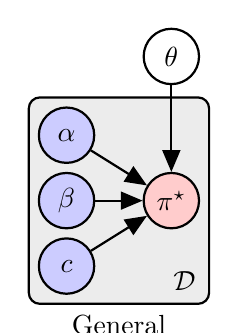
\begin{tikzpicture}[every path/.style={thick}]
  \tikzstyle{obs} = [latent,fill=blue!20];
  \tikzset{plate caption/.append style={below right=-.3cm and -.35cm of #1.south east}};
  \node[obs] (alpha) {$\alpha$};
  \node[obs,below=.1cm of alpha] (beta) {$\beta$};
  \node[obs,below=.1cm of beta] (c) {$c$};
  \node[obs,right=.6cm of beta,fill=red!20] (pi) {$\pi^\star$};
  \node[latent,above=1.1cm of pi] (theta) {$\theta$};
  \scoped[on background layer]{
    \plate [inner sep=.1cm,fill=gray!15] {plate} {(alpha) (beta) (c) (pi)} {};
  };
  \edge {alpha,beta,c} {pi};
  \edge {theta} {pi};
  \node[below right=-5.5mm and -6mm of plate.south east] {$\gD$};
  \begin{pgfinterruptboundingbox}
    \node[below=0mm of plate.south] {General};
  \end{pgfinterruptboundingbox}
\end{tikzpicture}
\hfill
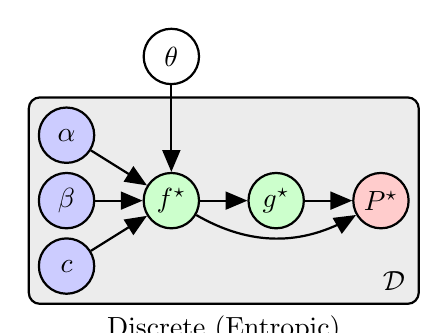
\begin{tikzpicture}[every path/.style={thick}]
  \tikzstyle{obs} = [latent,fill=blue!20];
  \tikzset{plate caption/.append style={below right=-.3cm and -.35cm of #1.south east}};
  \node[obs] (alpha) {$\alpha$};
  \node[obs,below=.1cm of alpha] (beta) {$\beta$};
  \node[obs,below=.1cm of beta] (c) {$c$};
  \node[obs,right=.6cm of beta,fill=green!20] (f) {$f^\star$};
  \node[obs,right=.6cm of f,fill=green!20] (g) {$g^\star$};
  \node[obs,right=.6cm of g,fill=red!20] (P) {$P^\star$};
  \node[latent,above=1.1cm of f] (theta) {$\theta$};
  \scoped[on background layer]{
    \plate [inner sep=.1cm,fill=gray!15] {plate} {(alpha) (beta) (c) (f) (g) (P)} {};
  };
  \edge {alpha,beta,c} {f};
  \edge {theta} {f};
  \edge {f} {g};
  \edge {g} {P};
  \draw[->] (f) to [out=-30,in=-150] (P);
  \node[below right=-5.5mm and -6mm of plate.south east] {$\gD$};
  \begin{pgfinterruptboundingbox}
    \node[below=0mm of plate.south] {Discrete (Entropic)};
  \end{pgfinterruptboundingbox}
\end{tikzpicture}
\hfill
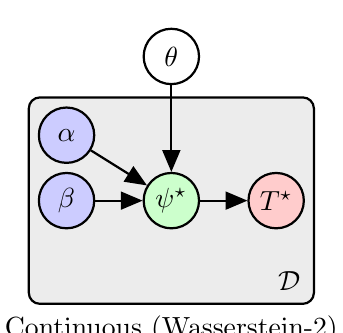
\begin{tikzpicture}[every path/.style={thick}]
  \tikzstyle{obs} = [latent,fill=blue!20];
  \tikzset{plate caption/.append style={below right=-.3cm and -.35cm of #1.south east}};
  \node[obs] (alpha) {$\alpha$};
  \node[obs,below=.1cm of alpha] (beta) {$\beta$};
  \node[obs,below=.1cm of beta,draw=none,fill=none] (c) {};
  \node[obs,right=.6cm of beta,fill=green!20] (psi) {$\psi^\star$};
  \node[obs,right=.6cm of psi,fill=red!20] (T) {$T^\star$};
  \node[latent,above=1.1cm of psi] (theta) {$\theta$};
  \scoped[on background layer]{
    \plate [inner sep=.1cm,fill=gray!15] {plate} {(alpha) (beta) (c) (psi) (T)} {};
  };
  \node[below right=-5.5mm and -6mm of plate.south east] {$\gD$};
  \edge {alpha,beta} {psi};
  \edge {theta} {psi};
  \edge {psi} {T};
  \begin{pgfinterruptboundingbox}
    \node[below=0mm of plate.south] {Continuous (Wasserstein-2)};
  \end{pgfinterruptboundingbox}
\end{tikzpicture} \\[6mm]
\circlegend{{blue!20}}{Input measures and cost} \hspace{2mm}
\circlegend{{green!20}}{Dual potentials} \hspace{2mm}
\circlegend{{red!20}}{Couplings}

%%% Local Variables:
%%% coding: utf-8
%%% mode: latex
%%% TeX-master: "meta-ot"
%%% End:

  \caption{
    Meta OT uses objective-based amortization for optimal transport.
    In the general formulation, the \emph{parameters} $\theta$ capture
    shared structure in the \emph{optimal couplings} $\pi^\star$ between
    multiple input measures and costs over some \emph{distribution} $\gD$.
    In practice, we learn this shared structure over the
    \emph{dual potentials} which map back to the coupling:
    $f^\star$ in discrete settings and $\psi^\star$ in continuous ones.
  }
  \label{fig:meta-OT}
\end{figure}

\Cref{fig:meta-OT} illustrates our key contribution of connecting
objective-based amortization in \cref{eq:amor-obj-opt} to
optimal transport. We consider solving \emph{multiple} OT problems
and learning shared structure and correlations between them.
We denote a joint \emph{meta-distribution} over the input
measures and costs with $\gD(\alpha,\beta,c)$, which we call \emph{meta}
to distinguish it from the measures $\alpha,\beta$.

In general, we could introduce a model that directly predicts
the primal solution to \cref{eq:kantorovich-primal}, \ie
$\pi_\theta(\alpha, \beta, c)\approx \pi^\star(\alpha, \beta, c)$
for $(\alpha, \beta, c)\sim \gD$.
This is difficult for the same reason why most computational methods
do not operate directly in the primal space: the optimal coupling
is often a high-dimensional joint distribution with
non-trivial marginal constraints.
We instead turn to predicting the dual variables used by today's solvers.

\subsection{Meta OT between discrete measures}
\label{sec:meta-ot:discrete}

We build on standard methods for entropic OT
reviewed in \cref{sec:prelim:discrete} between discrete measures
$\alpha \defeq \sum_{i=1}^m a_i \delta_{x_i}$ and $\beta \defeq \sum_{i=1}^n b_i \delta_{x_i}$
with $a \in \Delta_{m-1}$ and $b\in \Delta_{n-1}$
coupled using a cost $c$.
In the Meta OT setting, the measures and cost are the contexts for
amortization and sampled from a
\emph{meta-distribution}, \ie $(\alpha,\beta,c)\sim\gD(\alpha,\beta,c)$.
For example, \cref{sec:exp:mnist,sec:exp:world} considers meta-distributions
over the weights of the atoms, \ie $(a,b)\sim\gD$, where
$\gD$ is a distribution over $\Delta_{m-1} \times \Delta_{n-1}$.
\looseness=-1

\textbf{Amortization objective.}
We will seek to predict the \emph{optimal} potential.
At optimality, the pair of potentials are related to each
other via \cref{eq:f-to-g}, \ie
$g(f; \alpha, \beta, c) \defeq \epsilon \log b - \epsilon\log\left(K^\top \exp\{f/\epsilon\}\right)$
where $K\in\R^{m\times n}$ is the \emph{Gibbs kernel}
from \cref{eq:entropic-dual}.
Hence, it is sufficient to predict one of the
potentials, \eg $f$, and recover the other.
We thus re-formulate \cref{eq:entropic-dual}
to just optimize over $f$ with
\begin{equation}
  f^\star(\alpha, \beta, c, \epsilon)\in\ \argmin_{f\in\R^n}\ J(f; \alpha, \beta, c),
  \label{eq:entropic-dual-f}
\end{equation}
where $-J(f; \alpha, \beta, c)\defeq \langle f, a\rangle + \langle g, b \rangle$
is the dual objective over $f$.
Even though most solvers optimize over $f$ and $g$ jointly
as in \cref{eq:entropic-dual-f}, amortizing over these would likely need:
1) to have a higher capacity than a model just predicting $f$, and
2) to learn how $f$ and $g$ are connected through \cref{eq:f-to-g} while
in \cref{eq:entropic-dual-f} we explicitly provide this knowledge.

\textbf{Amortization model.}
We predict the solution to \cref{eq:entropic-dual-f} with
$\hat f_\theta(\alpha, \beta, c)$ parameterized by $\theta$, resulting in
a computationally efficient approximation $\hat f_\theta \approx f^\star$.
Here we use the notation $\hat f_\theta(\alpha,\beta,c)$ to mean that
the model $\hat f_\theta$ depends on \emph{representations} of
the input measures and cost.
In our settings, we define $\hat f_\theta$ as a fully-connected MLP
mapping from the atoms of the measures to the duals.

\textbf{Amortization loss.}
Applying objective-based amortization from \cref{eq:amor-obj-opt} to
the dual in \cref{eq:entropic-dual-f} completes our
learning setup. Our model should best-optimize the expectation of the dual objective
\begin{equation}
  \min_\theta \E_{(\alpha,\beta,c)\sim\gD} J(\hat f_\theta(\alpha, \beta, c); \alpha, \beta, c),
  \label{eq:amor-entropic-loss}
\end{equation}
which is appealing as it does not require ground-truth solutions $f^\star$.
\Cref{alg:meta-ot-training} shows a basic training loop for
\cref{eq:amor-entropic-loss} using a gradient-based
optimizer such as Adam \citep{kingma2014adam}.

\textbf{Sinkhorn fine-tuning.}
The dual prediction made by $\hat f_\theta$ with an associated $\hat g$
can easily be input as the initialization to a standard Sinkhorn solver
as shown in \cref{alg:sinkhorn-finetuning}.
This allows us to deploy the predicted potential with
Sinkhorn to obtain the optimal potentials with
only a few extra iterations.

\textbf{On accelerated solvers.}
Here we have only considered fine-tuning the Meta OT prediction
with a log-Sinkhorn solver.
Meta OT can also be combined with accelerated variants of
entropic OT solvers such as
\citet{thibault2017overrelaxed,altschuler2017near,alaya2019screening,lin2019acceleration}
that would otherwise solve every problem from scratch.


\textbf{Convergence rates.}
The knowledge of the hyper-distribution $\gD$ of problems
being solved enables Meta OT methods to surpass the
convergence rates and computational time of standard algorithms
by restricting the set of problems rather than considering
the average- or worst-case performance.
The model $\hat f_\theta$ distills information between the
problem instances into the parameters $\theta$.

\subsection{Meta OT between continuous measures (Wasserstein-2)}
\label{sec:meta-ot:icnn}
\begin{figure}[t]
% Copyright (c) Meta Platforms, Inc. and affiliates.

\begin{minipage}[t]{0.49\textwidth}
\begin{algorithm}[H]
    \caption{Training Meta OT}
    \begin{algorithmic}
    \footnotesize
    \State Initialize amortization model with $\theta_0$
    \For{iteration $i$}
    \State Sample $(\alpha, \beta, c)\sim\gD$
    \State Predict duals $\hat f_\theta$ or $\hat \varphi_\theta$ on the sample
    \State Estimate the loss in \cref{eq:amor-entropic-loss} or \cref{eq:amor-w2gn-loss}
    \State Update $\theta_{i+1}$ with a gradient step
    \EndFor
    \end{algorithmic}
    \label{alg:meta-ot-training}
\end{algorithm}
\end{minipage}
\hfill
\begin{minipage}[t]{0.49\textwidth}
\begin{algorithm}[H]
    \caption{Fine-tuning with Sinkhorn}
    \begin{algorithmic}
    \footnotesize
    \State Predict duals $\hat f_\theta(\alpha, \beta, c)$
    \State Compute $\hat g$ from $\hat f_\theta$ using \cref{eq:f-to-g}
    \State \Return Sinkhorn($\alpha, \beta, c, \epsilon, \hat f_\theta, \hat g$)
    \end{algorithmic}
    \label{alg:sinkhorn-finetuning}
\end{algorithm}
\vspace*{-5mm}
\begin{algorithm}[H]
    \caption{Fine-tuning with W2GN}
    \begin{algorithmic}
    \footnotesize
    \State Predict dual ICNN parameters $\hat \varphi_\theta(\alpha, \beta, c)$
    \State \Return W2GN($\alpha, \beta, c, T, \hat \varphi_\theta$)
    \end{algorithmic}
    \label{alg:w2gn-finetuning}
\end{algorithm}
\end{minipage}

%%% Local Variables:
%%% coding: utf-8
%%% mode: latex
%%% TeX-master: "meta-ot"
%%% End:

\end{figure}

We take an analogous approach to predicting the Wasserstein-2
map between continuous measures for Wasserstein-2 as reviewed in
\cref{sec:prelim:continuous}.
Here the measures $\alpha,\beta$ are supported in continuous space
$\gX=\gY=\R^d$ and we focus on computing Wasserstein-2 couplings
from instances sampled from a \emph{meta-distribution}
$(\alpha,\beta)\sim\gD(\alpha,\beta)$.
The cost $c$ is not included in $\gD$ as it remains fixed to the
squared Euclidean cost everywhere here.

One challenge here is that the optimal dual potential
$\psi^\star(\ \cdot\ ; \alpha, \beta)$
in \cref{eq:W2-dual} is a convex function and not simply
a finite-dimensional real vector.
The dual potentials in this setting are approximated by, \eg, an ICNN.
We thus propose a \emph{Meta ICNN} that predicts the \emph{parameters}
$\varphi$ of an ICNN $\psi_\varphi$ that approximates the optimal
dual potentials, which can be seen as a hypernetwork
\citep{stanley2009hypercube,ha2016hypernetworks}.
The dual prediction made by $\hat \varphi_\theta$
can easily be input as the initial value to a standard W2GN solver
as shown in \cref{alg:w2gn-finetuning}.
\Cref{app:other-W2-models} discusses other modeling
choices we considered: we tried models based on
MAML \citep{pmlr-v70-finn17a} and neural processes
\citep{garnelo2018neural,garnelo2018conditional}.

\textbf{Amortization objective.}
We build on the W2GN formulation \citep{korotin2019wasserstein}
and seek parameters $\varphi^\star$ optimizing the
dual ICNN potentials $\psi_\varphi$ and $\overline{\psi_\varphi}$
with $\gL(\varphi; \alpha, \beta)$ from \cref{eq:w2gn-loss}.
We chose W2GN due to the stability, but could also easily
use other losses optimizing ICNN potentials.

\textbf{Amortization model: the Meta ICNN.}
We predict the solution to \cref{eq:w2gn-loss} with
$\hat \varphi_\theta(\alpha, \beta)$ parameterized by $\theta$,
resulting in a computationally efficient approximation to
the optimum $\hat \varphi_\theta \approx \varphi^\star$.
\Cref{fig:meta-icnn} instantiates a convolutional Meta ICNN
model using a ResNet-18 \citep{he2016identity} architecture for
coupling image-based measures.
We again emphasize that $\alpha,\beta$ used with the model
here are \emph{representations} of measures, which in our cases are simply images.

\textbf{Amortization loss.}
Applying objective-based amortization from \cref{eq:amor-obj-opt} to
the W2GN loss in \cref{eq:w2gn-loss} completes our learning setup.
Our model should best-optimize the expectation of the loss:
\begin{equation}
  \min_\theta \E_{(\alpha,\beta)\sim\gD}
    \gL(\hat \varphi_\theta(\alpha, \beta); \alpha, \beta).
  \label{eq:amor-w2gn-loss}
\end{equation}
As in the discrete setting, it does not require ground-truth
solutions $\varphi^\star$ and we learn it with Adam.

\begin{figure}[t]
  \centering
  \vspace{-2mm}
  \begin{minipage}[t]{0.49\linewidth}
    \centering
    {\large Sinkhorn \color{gray}{(converged, ground-truth)}} \\
    \begin{tikzpicture}[every path/.style={thick}]
      \node[align=left,anchor=south west] {
\includegraphics[height=23px]{fig/mnist-interp-true.png}};
      \node at (2.6mm,0) (alpha) {\large$\alpha_0$};
      \node at (36mm,-2mm) {\large$\alpha_1$};
      \draw[line width=.5mm] (36mm,0mm) -- (36mm,2mm);
      \node at (64.5mm,0) (beta) {\large$\alpha_2$};
      \edge[<->] {alpha} {beta};
    \end{tikzpicture}
  \end{minipage}
  \hfill
  \begin{minipage}[t]{0.49\linewidth}
    \centering
    {\large Meta OT \color{gray}{(initial prediction)}} \\
    \begin{tikzpicture}[every path/.style={thick}]
      \node[align=left,anchor=south west] {
\includegraphics[height=23px]{fig/mnist-interp-pred.png}};
      \node at (2.6mm,0) (alpha) {\large$\alpha_0$};
      \node at (35mm,-2mm) {\large$\alpha_1$};
      \draw[line width=.5mm] (35mm,0mm) -- (35mm,2mm);
      \node at (64mm,0) (beta) {\large$\alpha_2$};
      \edge[<->] {alpha} {beta};
    \end{tikzpicture}
  \end{minipage}
  \caption{
    Interpolations between MNIST test digits using
    couplings obtained from
    (left) solving the problem with Sinkhorn, and
    (right) Meta OT model's initial prediction, which
    is $\bf{\approx}100$ times computationally cheaper and produces a nearly identical coupling.
  }
  \label{fig:mnist-test-vis}
\end{figure}

\begin{figure}[t]
  \centering
  \begin{tikzpicture}[every path/.style={thick}]
    \node (im1) {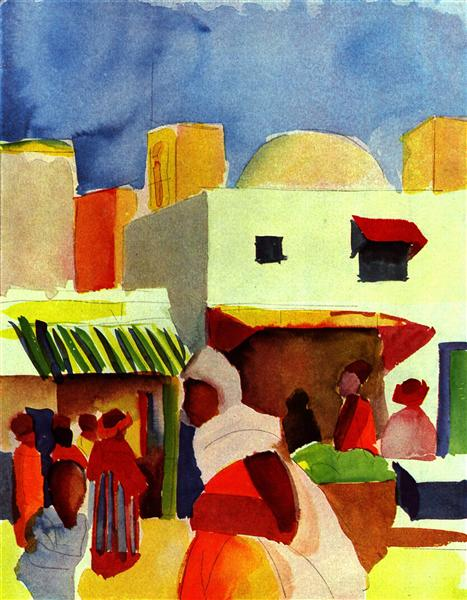
\includegraphics[width=.5in]{fig/color/market-in-algiers.jpg}};
    \node[below=0 of im1] (im2) {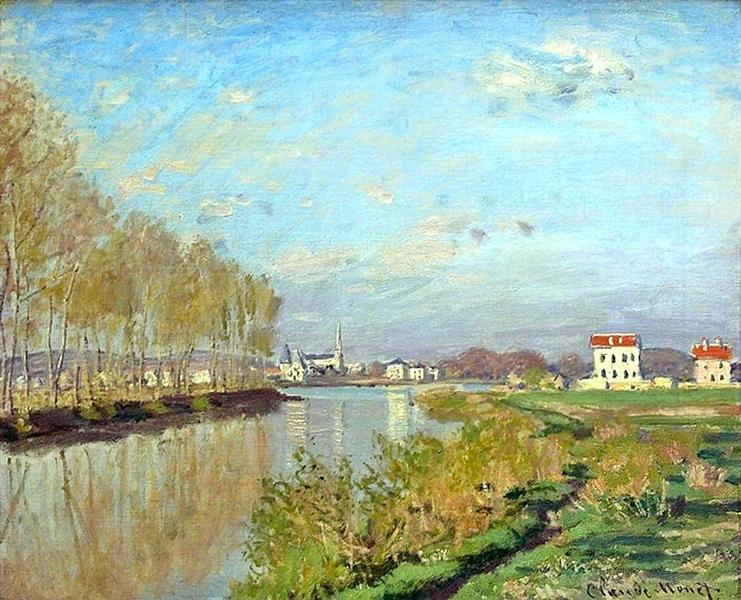
\includegraphics[width=.5in]{fig/color/argenteuil-the-seine.jpg}};
    \node[left=0 of im1] (alpha) {$\alpha$};
    \node[left=0 of im2] (beta) {$\beta$};
    \node[right=2cm of im1] (z1) {$z_1$};
    \node[right=2cm of im2] (z2) {$z_2$};
    \node[above=4.5mm of z1] () {$z$};
    \node[xshift=2.5mm] (zmid) at (barycentric cs:z1=1,z2=1) {};
    \path[draw,-] ($(zmid)+(.2mm,0)$) -- ($(zmid)+(-5mm,0)$);
    \scoped[on background layer]{
        \draw[fill=violet!20] ($(zmid) + (-5mm,-15mm)$) rectangle ($(zmid) + (0mm,+15mm)$);
    }
    \node[fill=green!20,draw=black,right=1.5cm of zmid] (varphi) {$\hat \varphi_\theta$};
    \node[below=0mm of varphi] () {Parameters};
    \node[fill=green!20,draw=black,right=1.5cm of varphi] (icnn) {$\psi_{\hat \varphi_\theta}$};
    \node[below=0mm of icnn] () {ICNN};
    \node[fill=red!20,draw=black,right=1.5cm of icnn] (icnn_grad) {$\hat T(\cdot)=\nabla_x\psi_{\hat \varphi_\theta}(\cdot)$};
    \node[below=0mm of icnn_grad] () {Transport map};
    \path[draw,->] (im1) -- node[above]{ResNet$_\theta$} (z1);
    \path[draw,->] (im2) -- node[above]{ResNet$_\theta$} (z2);
    \path[draw,->] (zmid) -- node[above]{MLP$_\theta$} (varphi);
    \edge[] {varphi} {icnn};
    \edge[] {icnn} {icnn_grad};
  \end{tikzpicture} \\[-1.5mm]
  \caption{A Meta ICNN for image-based input measures.
    A shared ResNet processes the input measures
    $\alpha$ and $\beta$ into latents $z$ that are decoded
    with an MLP into the parameters $\varphi$ of an ICNN dual
    potential $\psi_\varphi$.
    The derivative of the ICNN provides the transport map $\hat T$.
  }
  \label{fig:meta-icnn}
\end{figure}

\begin{figure}[t!]
  \centering
  \newcommand{\pair}[2]{$#1$ {\color{gray}\footnotesize $\pm#2$}}
  \hspace*{-3mm}
  \begin{minipage}{0.50\linewidth}
    \centering
    \vspace{5mm}
    \begin{table}[H]
      \vspace{-6mm}
      \centering
      \caption{Discrete OT runtime (in seconds) to reach a marginal error of $10^{-3}$
      and Meta OT's runtime.}
      \resizebox{\linewidth}{!}{
      \begin{tabular}{lccc} \toprule
        & MNIST & Spherical \\\midrule
        Sinkhorn & \pair{3.3\cdot10^{-3}}{1.0\cdot10^{-3}} & \pair{1.5}{0.64} \\
        Meta OT + Sinkhorn & \cellhi\pair{2.2\cdot10^{-3}}{3.8\cdot10^{-4}} & \cellhi \pair{0.48}{.24} \\ \midrule
        Meta OT (Initial prediction) & \pair{4.6\cdot10^{-5}}{2.8\cdot10^{-6}} & \pair{4.4\cdot10^{-5}}{3.2\cdot10^{-6}} \\
        \bottomrule
      \end{tabular}}
      \label{tab:discrete-runtime}
    \end{table}
  \end{minipage}
  \hfill
  \begin{minipage}{0.50\linewidth}
    \centering
    \begin{table}[H]
      \centering
      \caption{Color transfer runtimes and values.}
      \resizebox{\linewidth}{!}{
        \begin{tabular}{rlll} \toprule
          & Iter & Runtime (s) & Dual Value \\\midrule
Meta OT & None & \pair{3.5\cdot10^{-3}}{2.7\cdot10^{-4}} & \pair{0.90}{6.08\cdot10^{-2}} \\
+ W2GN & 1k & \pair{0.93}{2.27\cdot10^{-2}} & \pair{1.0}{2.57\cdot10^{-3}} \\
& 2k & \pair{1.84}{3.78\cdot10^{-2}} & \pair{1.0}{5.30\cdot10^{-3}} \\ \midrule
W2GN & 1k & \pair{0.90}{1.62\cdot10^{-2}} & \pair{0.96}{2.62\cdot10^{-2}} \\
& 2k & \pair{1.81}{3.05\cdot10^{-2}} & \pair{0.99}{1.14\cdot10^{-2}} \\
          \bottomrule
        \end{tabular}}
      \label{tab:color-runtimes}
    \end{table}
  \end{minipage}
  {\footnotesize We report the mean and {\color{gray}(standard deviation)} across 10 test instances.}\vspace{-3mm}
\end{figure}

\section{Experiments}\label{sec:experiments}
We demonstrate how Meta OT models improve the convergence
of the state-of-the-art solvers in settings where
solving multiple OT problems naturally arises.
We implemented our code in JAX \citep{jax2018github} as an
extension to the the Optimal Transport Tools (OTT)
package \citep{cuturi2022optimal}.
All experiments take roughly $\approx$2 hours to
run on our single Quadro GP100 GPU.
\Cref{app:exp-details} covers further experimental
and implementation details.
The source code to reproduce all of our experiments is available at
\url{http://github.com/facebookresearch/meta-ot}.

\subsection{Discrete OT between MNIST digits}
\label{sec:exp:mnist}
Images provide a natural setting for Meta OT where the
distribution over images provide the meta-distribution
$\gD$ over OT problems.
Given a pair of images $\alpha_0$ and
$\alpha_1$, each grayscale image is cast as a discrete measure
in 2-dimensional space where the intensities define the probabilities of the atoms.
The goal is to compute the optimal transport interpolation between the
two measures as in, \eg, \citet[\S7]{peyre2019computational}.
Formally, this means computing the optimal coupling $P^\star$
by solving the entropic optimal transport problem between $\alpha_0$ and
$\alpha_1$ and computing the interpolates as
$\alpha_t = (t\proj_y+(1-t)\proj_x) _{\#}P^\star$, for $t\in [0,1]$,
where $\proj_x(x,y)\defeq x$ and $\proj_y(x,y)=y$.
We selected $\epsilon=10^{-2}$ as \cref{app:mnist-eps} shows that
it gives interpolations that are not too blurry or sharp.

Our Meta OT model $\hat f_\theta$ (\cref{sec:meta-ot:discrete})
is an MLP that predicts the transport map between pairs of MNIST digits.
We train on every pair from the standard training dataset.
\Cref{fig:mnist-test-vis} shows that even without fine-tuning,
Meta OT's predicted Wasserstein interpolations between
the measures are close to the ground-truth interpolations
obtained from running the Sinkhorn algorithm to convergence.
We then fine-tune Meta OT's prediction with Sinkhorn as in
\cref{alg:sinkhorn-finetuning}.
\Cref{fig:discrete-errs} shows that the near-optimal predictions
can be quickly refined in fewer iterations than running
Sinkhorn with the default initialization,
and \cref{tab:discrete-runtime} shows the runtime required
to reach the default threshold.

\begin{figure}[t]
  \centering
  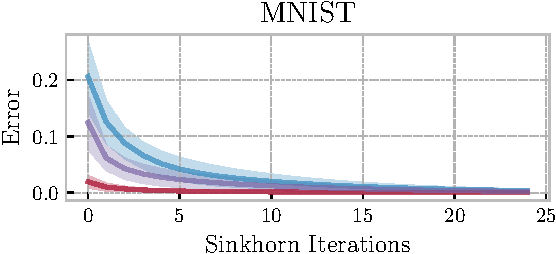
\includegraphics[width=0.49\textwidth]{fig/mnist-errs.pdf}
  \hfill
  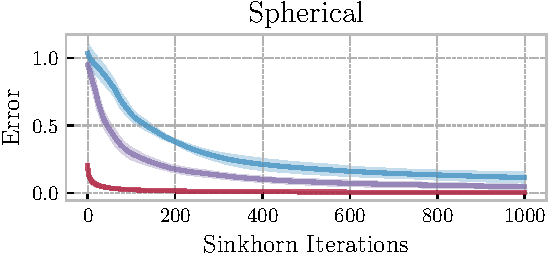
\includegraphics[width=0.49\textwidth]{fig/world-errs.pdf}
  \cblock{52}{138}{189} Sinkhorn \hspace{2mm}
  \cblock{166}{6}{40} Meta OT + Sinkhorn
  \caption{Sinkhorn convergence on test instances.
    Meta OT successfully predicts warm-start initializations
    that significantly improve the convergence of Sinkhorn iterations.
  }
  \label{fig:discrete-errs}
\end{figure}

\begin{figure}[t]
  \centering
  \begin{minipage}{0.45\linewidth}
    \centering
    {\large Sinkhorn \color{gray}{(converged, ground-truth)}} \\
    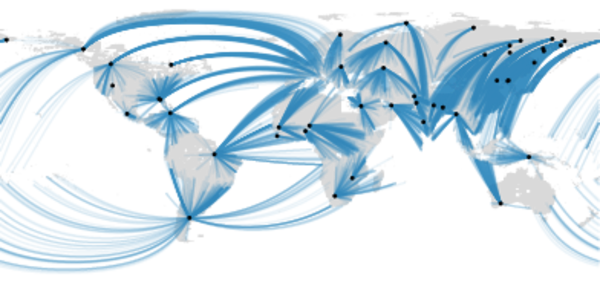
\includegraphics[width=\textwidth]{{fig/world/truth.0}.png} \\[-5mm]
    
\includegraphics[width=\textwidth]{{fig/world/truth.1}.png} \\[-5mm]
  \end{minipage}
  \hfill
  \begin{minipage}{0.45\linewidth}
    \centering
    {\large Meta OT \color{gray}{(initial prediction)}} \\
    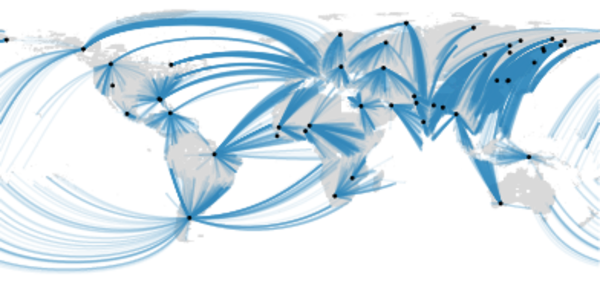
\includegraphics[width=\textwidth]{{fig/world/meta.0}.png} \\[-5mm]
    
\includegraphics[width=\textwidth]{{fig/world/meta.1}.png} \\[-5mm]
  \end{minipage}
  \caption{Test set coupling predictions of the spherical transport problem.
    Meta OT's initial prediction is $\bf{\approx}37500$ times faster
    than solving Sinkhorn to optimality.
    Supply locations are shown as black dots and the blue lines
    show the spherical transport maps $T$ going to demand locations
    at the end.
    The sphere is visualized with the Mercator projection.
  }
  \label{fig:world-errs}
\end{figure}

\newpage
\subsection{Discrete OT for supply-demand transportation on spherical data}
\label{sec:exp:world}

We next set up a synthetic transport problem between supply and demand
locations where the supply and demands may change locations or quantities
frequently, creating another Meta OT setting to be able to rapidly solve
the new instances.
We specifically consider measures living on the 2-sphere defined by
$\gS_2\defeq\{x\in\R^3: \|x\|=1\}$, \ie $\gX=\gY=\gS_2$,
with the transport cost given by the spherical distance
$c(x,y)=\arccos(\langle x, y \rangle)$.
We then randomly sample supply locations uniformly from Earth's
landmass and demand locations from Earth's population density to
induce a class of transport problems on the sphere
obtained from the CC-licensed dataset from \citet{doxsey2015taking}.
\Cref{fig:world-errs} shows that the predicted transport maps
on test instances are close to the optimal maps obtained from
Sinkhorn to convergence.
Similar to the MNIST setting, \cref{fig:discrete-errs,tab:discrete-runtime}
show improved convergence and runtime.

\begin{figure}[t]
  {\Large \hspace{.4in} $\alpha$ \hspace{1.35in} $\beta$ \hspace{.9in} $T_\#\alpha$ \hspace{1in} $T_\#^{-1}\beta$} \\
  \begin{tikzpicture}[node/.style={inner sep=0,outer sep=0}]
    \node[align=left,anchor=north west] {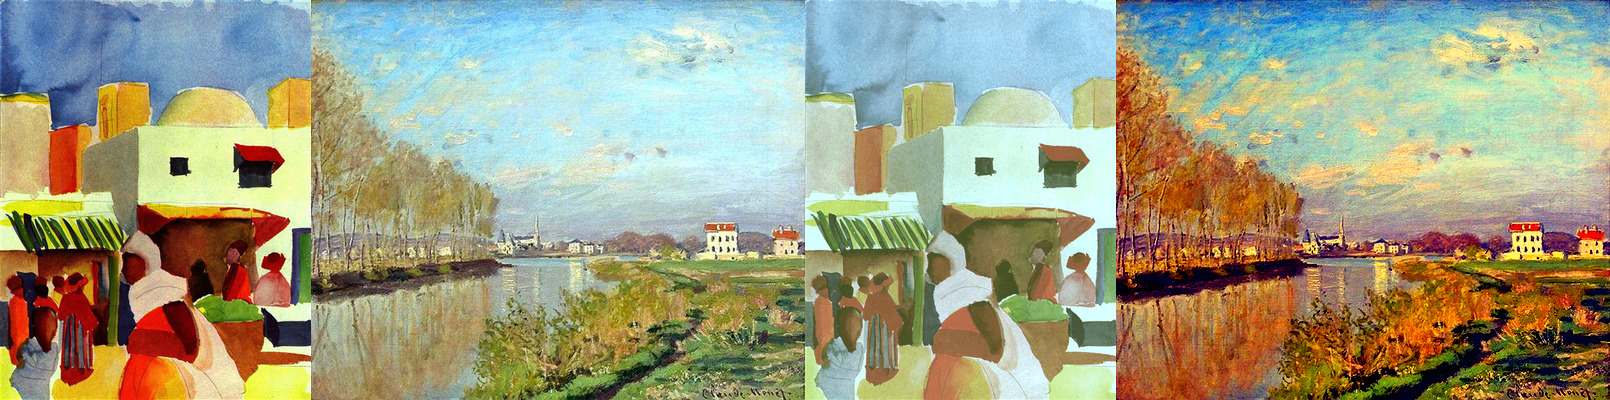
\includegraphics[width=\textwidth]{fig/color/val/0000_vanilla_final.jpg}};
    \node[fill=white, opacity=0.75, anchor=north west,inner sep=1mm] at (0,-1mm) {W2GN \color{black!80}{(converged, ground-truth)}};
  \end{tikzpicture} \\[-2.7mm]
  \begin{tikzpicture}[node/.style={inner sep=0,outer sep=0}]
    \node[align=left,anchor=north west] {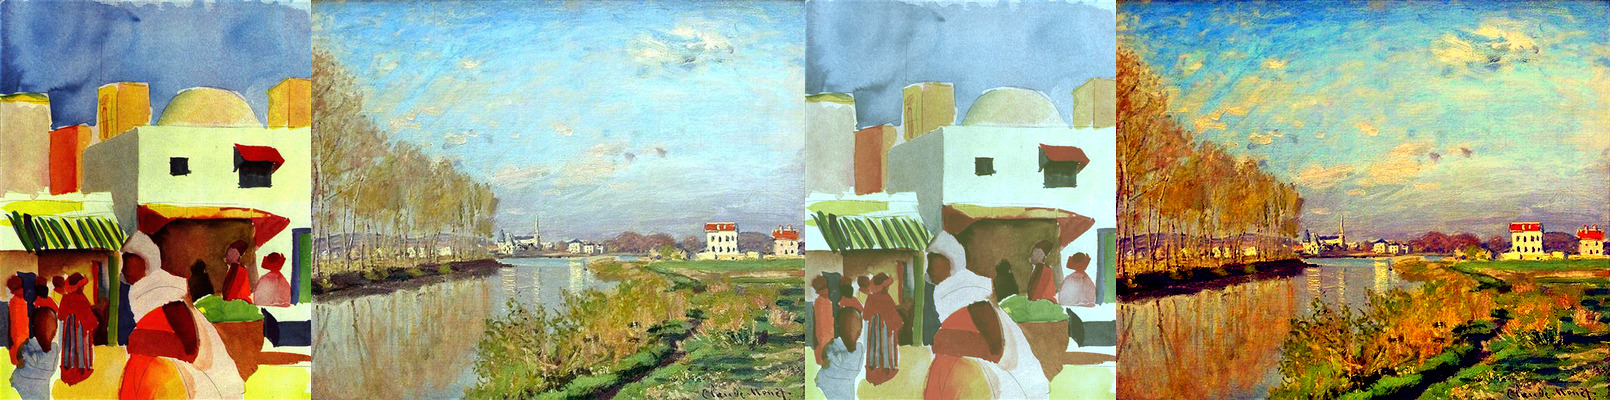
\includegraphics[width=\textwidth]{fig/color/val/0000_meta_init.jpg}};
    \node[fill=white, opacity=0.75, anchor=north west,inner sep=1mm] at (0,-1mm) {Meta OT \color{black!80}{(Initial prediction)}};
  \end{tikzpicture}
  \caption{Color transfers with a Meta ICNN on test pairs of images.
    The objective is to optimally transport the continuous RGB measure
    of the first image $\alpha$ to the second $\beta$,
    producing an invertible transport map $T$.
    Meta OT's prediction is $\bf{\approx}1000$ times faster
    than training W2GN from scratch.
    The image generating $\alpha$ is
    \href{https://www.wikiart.org/en/august-macke/market-in-algiers}{Market in Algiers by August Macke (1914)}
    and
    $\beta$ is
    \href{https://www.wikiart.org/en/claude-monet/argenteuil-the-sein}{Argenteuil, The Seine by Claude Monet (1872)},
    obtained from
    \href{https://www.wikiart.org/}{WikiArt}.
  }
  \label{fig:transfer-test-images}
\end{figure}


\subsection{Continuous Wasserstein-2 color transfer}
\label{sec:exp:w2}
\begin{wrapfigure}{R}{0.48\textwidth}
  \centering
  \vspace{-5mm}
  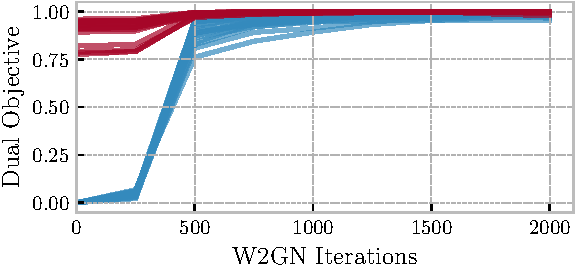
\includegraphics[width=0.5\textwidth]{fig/color/val-objs.pdf} \\
  \cblock{52}{138}{189} W2GN \hspace{2mm} \cblock{166}{6}{40} Meta OT + W2GN
  \caption{Convergence on color transfer test instances using W2GN.
    Meta ICNNs predicts warm-start initializations
    that significantly improve the (normalized) dual objective values.
  }
  \label{fig:transfer-convergence}
\end{wrapfigure}

The problem of color transfer between two images consists in mapping
the color palette of one image into the other one.
The images are required to have the same number of channels, for
example RGB images.
The continuous formulation that we use from \citet{korotin2019wasserstein},
takes \ie $\gX=\gY=[0,1]^3$ with $c$ being the squared Euclidean distance.
We collected ${\approx}200$ public domain images from
\href{https://www.wikiart.org/}{WikiArt}
and trained a Meta ICNN model from \cref{sec:meta-ot:icnn}
to predict the color transfer maps between every pair of them.
\Cref{fig:transfer-test-images} shows the predictions on test pairs
and \cref{fig:transfer-convergence} shows the convergence in comparison
to the standard W2GN learning.
\Cref{tab:color-runtimes} reports runtimes and
\cref{app:color} shows additional results.

\section{Related work}\label{sec:related_work}
\textbf{Efficiently estimating OT maps.}
To compute OT maps with fixed cost between pairs of measures
efficiently, neural OT models
\citep{korotin2019wasserstein,li2020continuous,korotin2021neural,mokrov2021large,korotin2021continuous}
leverage ICNNs to estimate maps between continuous high-dimensional
measures given samples from these, and
\citet{litvinenko2021computing,scetbon2021low,forrow2019statistical,sommerfeld2019optimal,scetbon2021linear,muzellec2019subspace,bonet2021subspace}
leverage structural assumptions on coupling and cost matrices to reduce
the computational and memory complexity. In the meta-OT setting, we
consider learning to rapidly compute OT mappings between new pairs
measures. All these works can hence potentially benefit from an
acceleration effect by leveraging amortization similarly.

\textbf{Embedding measures where OT distances are discriminative.}
Effort has been invested in learning encodings/projections of measures
through a nested optimization problem, which aims to find
discriminative embeddings of the measures to be compared
\citep{pmlr-v84-genevay18a, deshpande2019max,nguyen2022amortized}.
While these works share an encoder and/or a projection across task
with the aim of leveraging more discriminative alignments (and hence
an OT distance with a metric different from the Euclidean metric), our
work differs in the sense that we find good initializations to solve
the OT problem itself with fixed cost more efficiently across tasks.

\textbf{Optimal transport and amortization.}
Few previous works in the OT literature leverage
amortization. \citet{courty2017learning} learn a latent space in which
the Wasserstein distance between the measure's embeddings is
equivalent to the Euclidean distance. Concurrent work
\citep{nguyen2022amortized} amortizes the estimation of the optimal
projection in the max-sliced objective, which differs from our work
where we instead amortize the estimation of the optimal coupling
directly. Also, \citet{lacombe2021learning} learns to predict
Wasserstein barycenters of pixel images by training a convolutional
networks that, given images as input, outputs their barycenters. Our
work is hence a generalization of this pixel-based work to general
measures -- both discrete and continuous. A limitation of
\citet{lacombe2021learning} is that it does not provide alignments, as
the amortization networks predicts the barycenter directly rather than
individual couplings.

\section{Conclusions, future directions, and limitations}
\label{sec:con}
We have presented foundations for modeling and learning to
solve OT problems with Meta OT by using amortized optimization
to predict optimal transport plans.
This works best in applications that require solving
multiple OT problems with shared structure.
We instantiated it to speed up entropic regularized optimal
transport and unregularized optimal transport with squared
cost by multiple orders of magnitude.
We envision extensions of the work in:
1) \textbf{Meta OT models}.
While we mostly consider models based on hypernetworks,
other meta-learning paradigms can be connected in,
and
2) \textbf{OT algorithms}. While we instantiated
models on top of log-Sinkhorn and W2GN, Meta OT
could be integrated with most other methods too.
3) \textbf{OT applications} that are computationally
expensive and repeatedly solved, \eg in multi-marginal
and barycentric settings, or for Gromov-Wasserstein
distances between metric-measure spaces.

\textbf{Limitations.}
While we have illustrated successful applications of Meta OT,
it is also important to understand the limitations:
1) \textbf{Meta OT does not make previously intractable
problems tractable.}
All of the baseline OT solvers we consider solve
our problems within milliseconds or seconds.
2) \textbf{Out-of-distribution generalization.}
Meta OT may not generate good predictions on instances
that are not close to the training OT problems from the
meta-distribution $\gD$ over the measures and cost.
If the model makes a bad prediction,
one fallback option is to re-solve the instance from scratch.


% \subsection*{Acknowledgments}
% We would like to thank
% Eugene Vinitsky,
% Mark Tygert,
% Mathieu Blondel,
% Maximilian Nickel, and
% Muhammad Izzatullah
% for insightful comments and discussions.
% The core set of tools in Python
% \citep{van1995python,oliphant2007python}
% enabled this work, including
% Hydra \citep{Yadan2019Hydra},
% JAX \citep{jax2018github},
% Matplotlib \citep{hunter2007matplotlib},
% numpy \citep{oliphant2006guide,van2011numpy},
% Optimal Transport Tools \citep{cuturi2022optimal},
% and pandas \citep{mckinney2012python}.

{\small
\bibliographystyle{plainnat}
\bibliography{refs}
}

\iffalse
\section*{Checklist}
\begin{enumerate}
\item For all authors...
\begin{enumerate}
  \item Do the main claims made in the abstract and introduction accurately reflect the paper's contributions and scope?
    \answerYes{We hope so}
  \item Did you describe the limitations of your work?
    \answerYes{In \cref{sec:con}}
  \item Did you discuss any potential negative societal impacts of your work?
    \answerNo{We do not immediately foresee any that our work would add
      that the broader optimal transport field doesn't already have}
  \item Have you read the ethics review guidelines and ensured that your paper conforms to them?
    \answerYes{}
\end{enumerate}


\textcolor{gray}{
\item If you are including theoretical results...
\textcolor{black}{(This is not a theory paper)}
\begin{enumerate}
  \item Did you state the full set of assumptions of all theoretical results?
    \answerNA{}
  \item Did you include complete proofs of all theoretical results?
    \answerNA{}
\end{enumerate}
}


\item If you ran experiments...
\begin{enumerate}
  \item Did you include the code, data, and instructions needed to
    reproduce the main experimental results (either in the supplemental
    material or as a URL)?
    \answerYes{}
  \item Did you specify all the training details (e.g., data splits,
    hyperparameters, how they were chosen)?
    \answerYes{}
  \item Did you report error bars (e.g., with respect to the random seed after running experiments multiple times)?
    \answerYes{We show results from multiple trials in most places}
  \item Did you include the total amount of compute and the type of
    resources used (e.g., type of GPUs, internal cluster, or cloud provider)?
    \answerYes{}
\end{enumerate}

\item If you are using existing assets (e.g., code, data, models) or
curating/releasing new assets...
\begin{enumerate}
  \item If your work uses existing assets, did you cite the creators?
    \answerYes{}
  \item Did you mention the license of the assets?
    \answerYes{}
  \item Did you include new assets either in the supplemental material or as a URL?
    \answerNo{}
  \item Did you discuss whether and how consent was obtained from people whose data you're using/curating?
    \answerNA{}
  \item Did you discuss whether the data you are using/curating
    contains personally identifiable information or offensive content?
    \answerNA{}
\end{enumerate}

\textcolor{gray}{
\item If you used crowdsourcing or conducted research with human subjects...
\begin{enumerate}
  \item Did you include the full text of instructions given to
    participants and screenshots, if applicable?
    \answerNA{}
  \item Did you describe any potential participant risks, with links
    to Institutional Review Board (IRB) approvals, if applicable?
    \answerNA{}
  \item Did you include the estimated hourly wage paid to participants
    and the total amount spent on participant compensation?
    \answerNA{}
\end{enumerate}
}

\end{enumerate}
\fi

\newpage
\appendix
\section{Selecting $\epsilon$ for MNIST}
\label{app:mnist-eps}
\begin{figure}[h]
  \centering
  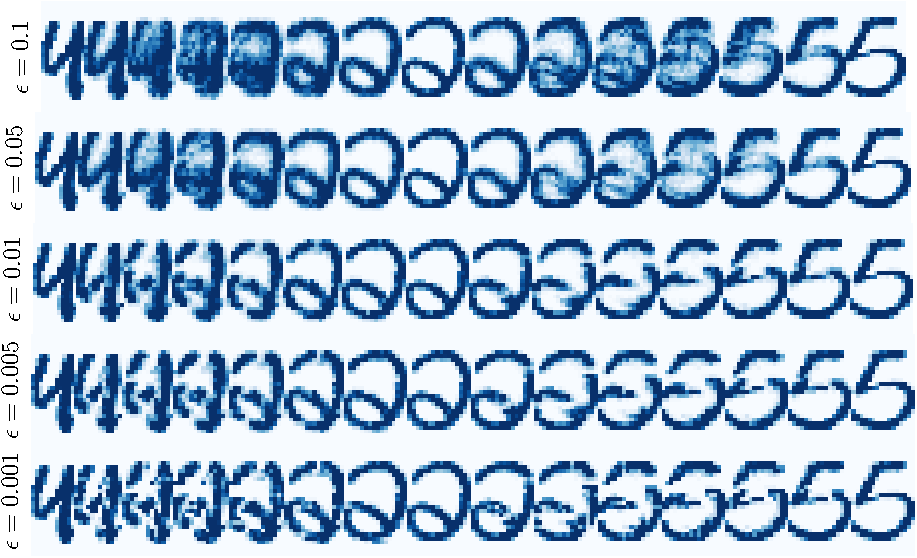
\includegraphics[width=\textwidth]{fig/mnist-epsilons.pdf}
  \caption{We selected $\epsilon=10^{-2}$ for our MNIST coupling
    experiments as it results in transport maps that are not
    too blurry or sharp.}
  \label{fig:mnist-epsilon}
\end{figure}

\section{Other models for continuous OT}
\label{app:other-W2-models}
While developing the hyper-network or Meta ICNN in \cref{sec:meta-ot:icnn}
for predicting couplings between continuous measures, we considered
alternative modeling formulations briefly documented in this section.
We finalized only the hyper-network model because it is conceptually the
most similar to predicting the optimal dual variables in the continuous setting
and results in rapid predictions.

\subsection{Optimization-based meta-learning (MAML-inspired)}
The model-agnostic meta-learning setup proposed in MAML \citep{pmlr-v70-finn17a}
could also be applied in the Meta OT setting to learn an adaptable
initial parameterization.
In the continuous setting, one initial version would take a parameterized
dual potential model $\psi_\varphi(x)$ and seek to learn an initial
parameterization $\varphi_0$ so that optimizing a loss such as the
W2GN loss $\gL$ from \cref{eq:w2gn-loss} results in a minimal
$\gL(\varphi_K)$ after adapting the model for $K$ steps.
Formally, this would optimize:
\begin{equation}
  \argmin_{\varphi_0} \gL(\varphi_K)\quad \text{where}\quad \varphi_{t+1}=\varphi_t-\nabla_\varphi\gL(\varphi_t)
  \label{eq:maml-meta-ot}
\end{equation}

\citet{tancik2021learned} explores similar learned initializations
for coordinate-based neural implicit representations for 2D images,
CT scan reconstruction, and 3d shape and scene recovery from 2D observations.

\textbf{Challenges for Meta OT.}
The transport maps given by $T=\nabla\psi$ can significantly
vary depending on the input measures $\alpha,\beta$.
We found it difficult to learn an initialization that can be rapidly
adapted, and optimizing \cref{eq:maml-meta-ot} is
more computationally expensive than
\cref{eq:amor-w2gn-loss} as it requires unrolling through many
evaluations of the transport loss $\gL$.
And, we found that \emph{only} learning to predict the optimal
parameters with \cref{eq:amor-w2gn-loss}, conditional on the input measures,
and then fine-tuning with W2GN to be stable.

\textbf{Advantages for Meta OT.}
Exploring MAML-inspired methods could further incorporate the knowledge
that the model's prediction is going to be fine-tuned into the
learning process.
One promising direction we did not try could be to integrate
some of the ideas from
LEO \citep{rusu2018meta} and CAVIA \citep{zintgraf2019fast},
which propose to learn a latent space for the parameters
where the initialization is also conditional on the input.

\subsection{Neural process}
The (conditional) neural process models considered in \citet{garnelo2018neural,garnelo2018conditional}
can also be adapted for the Meta OT setting.
In the continuous setting, this would result in a
dual potential that is also conditioned on a representation
of the input measures, \eg $\psi_\varphi(x; z)$ where
$z\defeq f^{\rm emb}_\varphi(\alpha, \beta)$ is a learned embedding
of the input measures that is learned with the parameters of $\psi$.
This could be formulated as
\begin{equation}
  \argmin_\varphi \E_{(\alpha,\beta)\sim\gD} \gL(\varphi, f^{\rm emb}_\varphi(\alpha, \beta)),
  \label{eq:neural-process-meta-ot}
\end{equation}
where $\gL$ modifies the model used in the loss \cref{eq:w2gn-loss} to
also be conditioned on the context extracted from the measures.

\textbf{Challenges for Meta OT.}
This raises the issue on best-formulating the model to be conditional
on the context. One way could be to append $z$ to the input
point $x$ in the domain, but if $\psi$ is an input-convex neural network,
then the model would only need to be convex with respect to $x$
and not $z$.
\looseness=-1

\textbf{Advantages for Meta OT.}
A large advantage is that the representation $z$ of the measures
$\alpha,\beta$ would be significantly lower-dimensional than the
parameters $\varphi$ that our Meta OT models are predicting.

\section{Additional experimental and implementation details}
\label{app:exp-details}

\iffalse
We have attached the Jax source code necessary to run and reproduce all
of the experiments in our paper and will open-source all of it.
Here is a basic overview of the files:

\newcommand{\fname}[2]{\texttt{#1} \quad #2}
\begin{forest}for tree={folder, grow'=0, inner sep=0pt,}, [
    [\fname{meta\_ot}{Meta OT Python library code}
      [\fname{conjugate.py}{Exact conjugate solver for the continuous setting}]
      [\fname{data.py}{}]
      [\fname{models.py}{}]
      [\fname{utils.py}{}]
    ]
    [\fname{config}{Hydra configuration for the experiments (containing hyper-parameters)}]
    [\fname{train\_discrete.py}{Train Meta OT models for discrete OT}]
    [\fname{train\_color\_single.py}{Train a single ICNN with W2GN between 2 images (for debugging)}]
    [\fname{train\_color\_meta.py}{Train a Meta ICNN with W2GN}]
    [\fname{plot\_mnist.py}{Visualize the MNIST couplings}]
    [\fname{plot\_world\_pair.py}{Visualize the spherical couplings}]
    [\fname{eval\_color.py}{Evaluate the Meta ICNN in the continuous setting}]
    [\fname{eval\_discrete.py}{Evaluate the Meta ICNN for the discrete tasks}]
  ]
\end{forest}

\newpage
Connecting to the data is one difficulty in running the experiments.
The easiest experiment to re-run is the MNIST one, which will automatically
download the dataset:

\begin{lstlisting}
./train_discrete.py # Train the model, outputting to <exp_dir>
./eval_discrete.py <exp_dir> # Evaluate the learned models
./plot_mnist.py <exp_dir> # Produce further visualizations
\end{lstlisting}
\fi

\subsection{Hyper-parameters}
We briefly summarize the hyper-parameters we used for training,
which we did not extensively tune.
In the discrete setting, we use the same hyper-parameters for the
MNIST and spherical settings.
\begin{table}[h]
  \caption{Discrete OT hyper-parameters.}
  \centering
  \begin{tabular}{rl}\toprule
    Name & Value \\\midrule
    Batch size & 128 \\
    Number of training iterations & 50000 \\
    MLP Hidden Sizes & [1024, 1024, 1024] \\
    Adam learning rate & 1e-3 \\\bottomrule
  \end{tabular}
\end{table}

\begin{table}[h]
  \caption{Continuous OT hyper-parameters.}
  \centering
  \begin{tabular}{rl}\toprule
    Name & Value \\\midrule
    Meta batch size (for $\alpha,\beta$) & 8 \\
    Inner batch size (to estimate $\gL$) & 1024 \\
    Cycle loss weight ($\gamma$) & 3. \\

    Adam learning rate & 1e-3 \\
    $\ell_2$ weight penalty & 1e-6 \\
    Max grad norm (for clipping) & 1. \\

    Number of training iterations & 200000 \\
    Meta ICNN Encoder & ResNet18 \\
    Encoder output size (both measures) & 256$\times$2 \\
    Meta ICNN Decoder Hidden Sizes & [512] \\\bottomrule
  \end{tabular}
\end{table}

\newpage
\section{Additional color transfer results}
\label{app:color}
We next show additional color transfer results
from the experiments in \cref{sec:exp:w2}
on the following public domain images from
\href{https://www.wikiart.org/}{WikiArt}:

\begin{itemize}
\item \href{https://www.wikiart.org/en/winston-churchill/distant-view-of-the-pyramids-1921}{Distant View of the Pyramids by Winston Churchill (1921)}
\item \href{https://www.wikiart.org/en/claude-monet/charing-cross-bridge-overcast-weather}{Charing Cross Bridge, Overcast Weather by Claude Monet (1900)}
\item \href{https://www.wikiart.org/en/claude-monet/houses-of-parliament}{Houses of Parliament by Claude Monet (1904)}
\item \href{https://www.wikiart.org/en/childe-hassam/october-sundown-newport-1901}{October Sundown, Newport by Childe Hassam (1901)}
\item \href{https://www.wikiart.org/en/juan-gris/landscape-with-house-at-ceret-1913}{Landscape with House at Ceret by Juan Gris (1913)}
\item \href{https://www.wikiart.org/en/claude-monet/irises-in-monet-s-garden-03}{Irises in Monet's Garden by Claude Monet (1900)}
\item \href{https://www.wikiart.org/en/paul-klee/crystal-1921}{Crystal Gradation by Paul Klee (1921)}
\item \href{https://www.wikiart.org/en/paul-klee/senecio-1922}{Senecio by Paul Klee (1922)}
\item \href{https://www.wikiart.org/en/josef-capek/vaza-s-kvetinami-1914}{Váza s květinami by Josef Capek (1914)}
\item \href{https://www.wikiart.org/en/vincent-van-gogh/sower-with-setting-sun-1888-3}{Sower with Setting Sun by Vincent van Gogh (1888)}
\item \href{https://www.wikiart.org/en/claude-monet/three-trees-in-grey-weather}{Three Trees in Grey Weather by Claude Monet (1891)}
\item \href{https://www.wikiart.org/en/vincent-van-gogh/vase-with-daisies-and-anemones-1887}{Vase with Daisies and Anemones by Vincent van Gogh (1887)}
\end{itemize}
\newpage

\def\photos{0004,0006,0007,0009,0010,0012}
\def\head{{\Large \hspace{.45in} $\alpha$ \hspace{1.2in} $\beta$ \hspace{1.0in} $T_\#\alpha$ \hspace{.9in} $T_\#^{-1}\beta$}}
\begin{figure}[H]
  \vspace{-.43in}
  \head \\
  \foreach \I in \photos {\includegraphics[width=\textwidth]{fig/color/val/\I_meta_init.jpg} \\}
  \caption{Meta ICNN (initial prediction).
    The sources are given in the beginning of \cref{app:color}.
  }
\end{figure}

\begin{figure}[H]
  \vspace{-.43in}
  \head \\
  \foreach \I in \photos {\includegraphics[width=\textwidth]{fig/color/val/\I_meta_final.jpg} \\}
  \caption{Meta ICNN + W2GN fine-tuning.
    The sources are given in the beginning of \cref{app:color}.}
\end{figure}

\begin{figure}[H]
  \vspace{-.43in}
  \head \\
  \foreach \I in \photos {\includegraphics[width=\textwidth]{fig/color/val/\I_vanilla_final.jpg} \\}
  \caption{W2GN (final). The sources are given in the beginning of \cref{app:color}.}
\end{figure}

\section{Out-of-distribution generalization}
In this experiment, we test the ability of our proposed approach to predict potentials for out-of-distribution input data. In particular, we consider the pairwise tests on 1) MNIST dataset used previously; 2) USPS dataset \citep{uspsdataset} upscaled to have the same size as the MNIST dataset; 3) Google Doodles dataset \footnote{\url{https://quickdraw.withgoogle.com/data}} with classes Crab, Cat and Faces; 4) sparsified random uniform data in [0,1] where sparsity (zeroing values below 0.95) is used to mimic the sparse signal in black-and-white images. For each pair, eg, MNIST-USPS, we train on one dataset and use the other to predict the potentials. The comparison is done using the same metric as before, ie, the deviation from the marginal constraints.  The results are presented in Figure \ref{fig:cross_domain}.

\begin{figure}[!t]
    \centering
    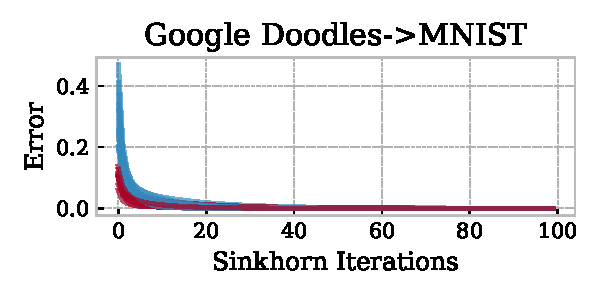
\includegraphics[width=.32\linewidth]{fig/cross_domain/errs_doodles_mnist.pdf}
    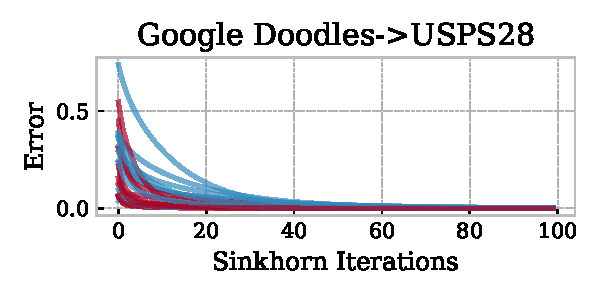
\includegraphics[width=.32\linewidth]{fig/cross_domain/errs_doodles_usps28.pdf}
    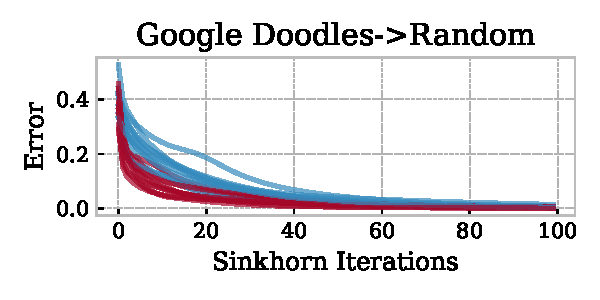
\includegraphics[width=.32\linewidth]{fig/cross_domain/errs_doodles_random.pdf}

    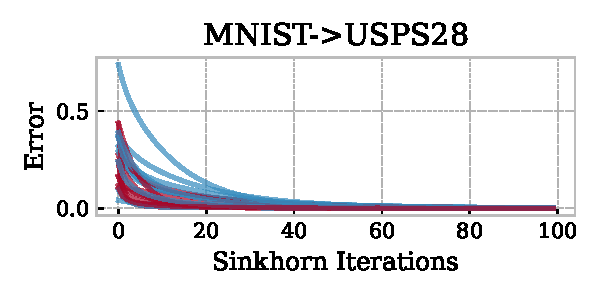
\includegraphics[width=.32\linewidth]{fig/cross_domain/errs_mnist_usps28.pdf}
    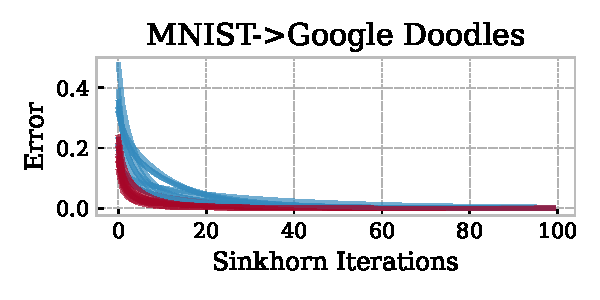
\includegraphics[width=.32\linewidth]{fig/cross_domain/errs_mnist_doodles.pdf}
    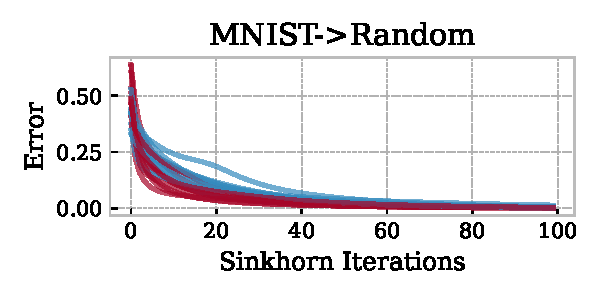
\includegraphics[width=.32\linewidth]{fig/cross_domain/errs_mnist_random.pdf}
    
    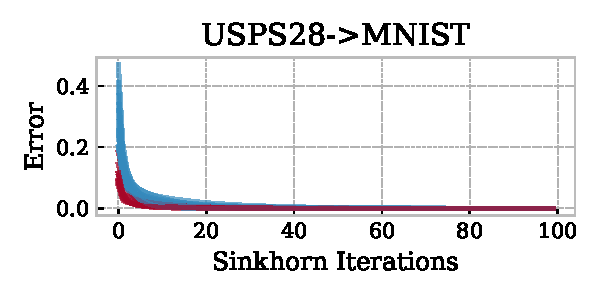
\includegraphics[width=.32\linewidth]{fig/cross_domain/errs_usps28_mnist.pdf}
    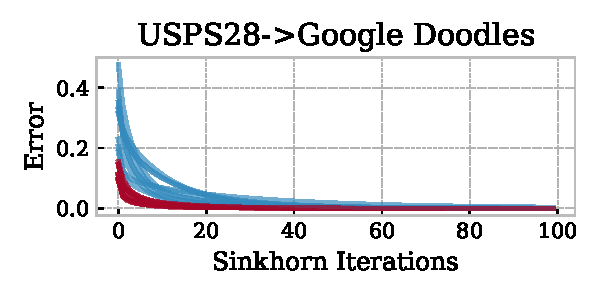
\includegraphics[width=.32\linewidth]{fig/cross_domain/errs_usps28_doodles.pdf}
    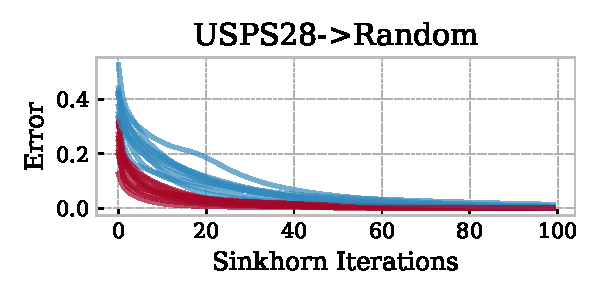
\includegraphics[width=.32\linewidth]{fig/cross_domain/errs_usps28_random.pdf}
    
    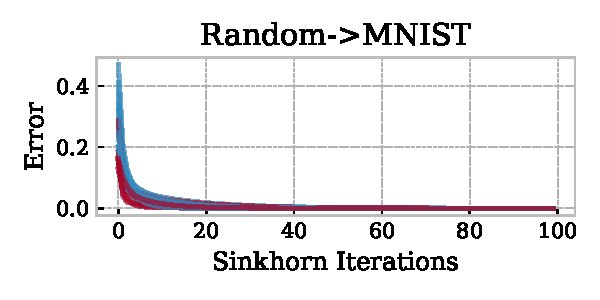
\includegraphics[width=.32\linewidth]{fig/cross_domain/errs_random_mnist.pdf}
    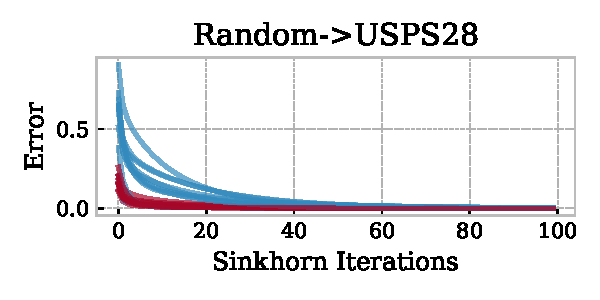
\includegraphics[width=.32\linewidth]{fig/cross_domain/errs_random_usps28.pdf}
    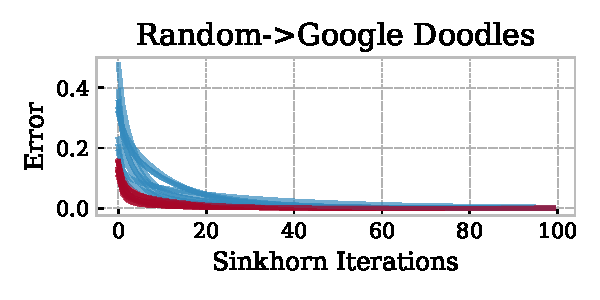
\includegraphics[width=.32\linewidth]{fig/cross_domain/errs_random_doodles.pdf}
    
    \label{fig:cross_domain}
    \caption{Cross-domain experiments}
\end{figure}

\end{document}
